\documentclass[12pt]{report}

% Uklonite ili komentirajte liniju koja uključuje kpfonts paket
%\usepackage[classicReIm]{kpfonts}

% Dodajte paket za Arial font
\usepackage{helvet}
\renewcommand{\familydefault}{\sfdefault}

% Dodajte paket za podešavanje proreda
\usepackage{setspace}

% Podešavanje proreda na 1,5 redak
\onehalfspacing

% Dodajte paket za podešavanje margina
\usepackage[a4paper, left=3cm, right=2.5cm, top=2.5cm, bottom=2.5cm]{geometry}

\usepackage[utf8]{inputenc}
%\usepackage[T1]{fontenc}
\usepackage[croatian]{babel}
\usepackage{amssymb}
\usepackage{amsmath}
\usepackage{txfonts}
\usepackage{mathdots}
\usepackage{titlesec}
\usepackage{array}
\usepackage{lastpage}
\usepackage{etoolbox}
\usepackage{tabularray}
\usepackage{color, colortbl}
\usepackage{adjustbox}
\usepackage{hyperref}
\usepackage{url}
\usepackage{fancyhdr}

\usepackage{float}
\usepackage{ragged2e}

\usepackage{comment}

\usepackage{listings}
\usepackage{xcolor}

% Dodavanje paketa za naslove tablica
\usepackage{caption}

% Oblik naslova poglavlja
\titleformat{\chapter}{\normalfont\huge\bfseries}{\thechapter.}{20pt}{\Huge}
\titlespacing{\chapter}{0pt}{0pt}{40pt}

\hypersetup{colorlinks, citecolor=black, filecolor=black, linkcolor=black, urlcolor=black}   % Izgled poveznice

% Prored smanjen između redaka u nabrajanjima i popisima
\newenvironment{packed_enum}{
    \begin{enumerate}
        \setlength{\itemsep}{0pt}
        \setlength{\parskip}{0pt}
        \setlength{\parsep}{0pt}
    }{\end{enumerate}}

\newenvironment{packed_item}{
    \begin{itemize}
        \setlength{\itemsep}{0pt}
        \setlength{\parskip}{0pt}
        \setlength{\parsep}{0pt}
    }{\end{itemize}}

% Boja za privatni i udaljeni ključ u tablicama
\definecolor{LightBlue}{rgb}{0.9,0.9,1}
\definecolor{LightGreen}{rgb}{0.9,1,0.9}

% Promjena teksta za dugačke tablice
\DefTblrTemplate{contfoot-text}{normal}{Nastavljeno na idućoj stranici}
\SetTblrTemplate{contfoot-text}{normal}
\DefTblrTemplate{conthead-text}{normal}{(Nastavljeno)}
\SetTblrTemplate{conthead-text}{normal}
\DefTblrTemplate{middlehead,lasthead}{normal}{Nastavljeno od prethodne stranice}
\SetTblrTemplate{middlehead,lasthead}{normal}

% Prilagodba stila sadržaja
\usepackage{tocloft}
\renewcommand{\cfttoctitlefont}{\normalfont\Large\bfseries}
\renewcommand{\cftsecfont}{\normalfont}
\renewcommand{\cftsecpagefont}{\normalfont}

% Dodavanje točkica u sadržaj
\renewcommand{\cftchapleader}{\cftdotfill{\cftdotsep}}
\renewcommand{\cftsecleader}{\cftdotfill{\cftdotsep}}
\renewcommand{\cftsubsecleader}{\cftdotfill{\cftdotsep}}

\begin{document}
    \pagenumbering{gobble} % Isključi brojeve stranica za početne stranice

    \newpage
    \thispagestyle{empty} % Prva prazna stranica
    \mbox{}

    \newpage
    \renewcommand{\contentsname}{Sadržaj} % Promjena naslova sadržaja
    \tableofcontents

    % Postavljanje brojača stranica na 1 i ponovno uključivanje brojeva stranica
    \cleardoublepage
    \pagenumbering{arabic}
    \setcounter{page}{1}

    % Uvod kao poglavlje 1
    \chapter*{Uvod}
\addcontentsline{toc}{chapter}{Uvod}
\noindent Polaganje vozačkog ispita dio je života gotovo svakog pojedinca. Prema nedavnim istraživanjima o zemljama u kojima je najteže i najskuplje naučiti voziti, Hrvatska se našla na vrhu rang-ljestvice. Procjenjuje se da je iznos koji vozači u Hrvatskoj moraju potrošiti kako bi položili sve ispite i dobili vozačku dozvolu oko 1085 eura. Kao razlog teškog polaganja vozačkog ispita se navode strogi uvjeti koji zahtijevaju veliku količinu učenja i praćenja napretka kandidata. Rješenje problema prijenosa znanja, organizacije izvođenja obuke i kontinuiranog praćenje svakog kandidata zahtjeva određenu razinu digitalizacije i implementaciju odgovarajuće aplikacije.\\

\noindent Cilj ovog završnog rada je kreiranje aplikacije "Vožnja +" čija je osnovna zadaća unapređenje vozačke obuke olakšavajući instruktorima i polaznicima autoškola  organizaciju i praćenje usvajanja vozačkih vještina. Kako bi korisnici dobili osnovne informacije i kontakt s autoškolom, anonimnim korisnicima omogućen je pristup stranicama s osnovnim informacijama i pristup formi za slanje upita. Svaki polaznik na raspolaganju ima vlastiti kalendar, korisnički profil i stranicu s napretkom koja sadrži bilješke za svaki sat koji je održan. Instruktori imaju pregled svih kandidata kojima mogu zakazivati termine ovisno o njihovoj raspoloživosti, a nakon održanog termina instruktor unosi bilješke za održani sat. Kalendari kandidata i instruktora automatski se sinkroniziraju te se tako može učinkovito organizirati i pratiti radno vrijeme instruktora. Aplikacija administratoru pruža mogućnost registracije novih korisnika te pregled svih korisnika i njihovih kalendara u sustavu. \\ 

\noindent U nastavku ovog rada slijedi detaljan opis korisničkih zahtjeva putem kojih će se definirati glavni zahtjevi i funkcionalnosti aplikacije "Vožnja +". Poglavlje o  dizajnu i arhitekturi sustava približit će čitatelju odabranu bazu podataka i implementaciju podatkovnog sloja, sloja poslovne logike i sloja korisničkog sučelja. Nakon implementacijskih detalja, bit će dan osvrt na korištene tehnologije. Za izradu web aplikacije korišteni su razvojni okviri Spring Boot i React, dok je za bazu korištena H2 baza podataka. Na kraju dolazi pregled korisničkih sučelja za sve vrste korisnika aplikacije.
    \chapter{Korisnički zahtjevi}
\section{Opis stranica}
\subsubsection{Početna stranica}
Pri pokretanju web aplikacije prikazuje se početna stranica koja pruža korisniku osnovne informacije o web aplikaciji te usmjerava korisnika na prijavu u sustav. U gornjem dijelu stranice nalazi se navigacijska traka putem koje korisnik pristupa različitim stranicama ovisno o svojim ovlastima. 
\subsubsection{Prijava}
Omogućuje korisniku unos korisničkih podataka i prijavu u aplikaciju pomoću adrese elektroničke pošte i lozinke. Korisnik se u sustav može samo prijaviti, registraciju novih korisnika obavlja administrator. Prijavljen korisnik neće moći pristupiti ovoj stranici.
\subsubsection{Info}
Pruža korisniku detaljnije informacije o autoškoli te približava svrhu same aplikacije. Stranica usmjerava korisnika na slanje upita putem kontaktnog obrasca ako ima dodatnih pitanja ili se želi prijaviti u autoškolu. Kontaktnim podacima može se pristupiti i u podnožju stranice.
\subsubsection{Kontakt}
Sadrži obrazac koji korisnik ispunjava pomoću imena, adrese elektroničke pošte i poruke. Ispunjen obrazac se šalje autoškoli klikom na gumb "Pošalji" koja se zatim javlja s odgovorima na potencijalna pitanja.
\subsubsection{Profil}
Prikazuje korisničke podatke unesene pri registraciji korisnika. Potrebni korisnički podaci za registraciju su ime, prezime, uloga, adresa elektroničke pošte, broj mobitela i datum rođenja. Osim obaveznih podataka, može se unijeti i napomena/bilješka za pojedinog korisnika koja se kasnije može uređivati i brisati.
\subsubsection{Kalendar}
Stranica namijenjena primarno instruktorima i polaznicima autoškole.Omogućuje prikaz, dodavanje, uređivanje i brisanje događaja u kalendar svakog korisnika. Na stranici se također nalaze korisničke upute za previđeno korištenje kalendara. Od kandidata se očekuje unos vremenske raspoloživosti prema kojoj instruktor unosi vrijeme obuke u raspored.
\subsubsection{Napredak}
Prikazuje napredak kandidata uz detaljan opis ishoda svakog sata. Realizirani ishod zabilježen je u posebnoj bilješci za svaki sat koju unosi instruktor putem forme na unos održanih sati. Klikom na pojedinu stavku iz trake za napredak prikazuje se skočni prozor sa svim detaljima za pojedini sat. Detalji koje korisnik može vidjeti su naslov održanog sata, datum, status, bilješka fotografija odvožene rute.
\subsubsection{Kandidati}
Stranica "Kandidati" pruža jednostavan pregled svih kandidata u autoškoli i omogućuje pristup podacima željenog kandidata. Podaci kojima instruktor i administrator mogu pristupiti su korisnički podaci sa stranice "Profil", kalendar i napredak željenog kandidata.
\subsubsection{Instruktori}
Omogućava  jednostavan pregled svih instruktora u autoškoli i omogućuje pristup podacima željenog instruktora. Podaci kojima administrator može pristupiti su korisnički podaci sa stranice "Profil"  i kalendar željenog instruktora.




\section{Vrste korisnika}
Postoje četiri kategorije korisnika sustava: neregistrirani korisnik te registrirani korisnici u koje ubrajamo  polaznike autoškole, instruktore i administratora.
\subsubsection{Anoniman korisnik}
Web aplikacija "Vožnja +" neregistriranom korisniku pruža pristup sljedećim stranicama: početna stranica, stranica za prijavu i informacije te stranici za slanje kontaktnog obrasca.  Korisnik može pronaći dodatne kontakt informacije i u podnožju stranice svake. Navedenim stranicama korisnik pristupa putem navigacijske trake.
\subsubsection{Kandidat}
Kao i anoniman korisnik, kandidat ima pristup početnoj stranici i stranici s dodatnim informacijama. Ako polaznik želi stupiti u kontakt s autoškolom, može to učiniti slanjem kontaktnog obrasca kojem pristupa preko stranice "Info" ili putem kontaktnih podataka u podnožju stranice. Na stranici "Profil" korisnik ima pregled svojih korisničkih podataka. Na toj stranici posebno se ističe mogućnost dodavanja i uređivanja bilješke ili napomene za svakog kandidata. Jedna od glavnih funkcionalnosti koje aplikacija pruža kandidatu je na stranici "Kalendar" gdje korisnik može dodavati, uređivati i brisati događaje što je posebno prikladno za označavanje vremenske raspoloživosti samog kandidata, a u istom kalendaru Korisnik može vidjeti termine koje mu je zakazao instruktor. Na stranici "Napredak" kandidat ima pristup traci za napredak putem koje se prati obuka kandidata. Klikom na odgovarajući element navigacijske trake, kandidatu je omogućen pregled bilješki za pojedini sat.
\subsubsection{Instruktor}
Poput kandidata, instruktor ima pristup početnoj stranici, kontaktnoj formi putem stranice "Info", stranici "Profil" s korisničkim podacima i stranici s vlastitim kalendarom. Dodatna mogućnost koju aplikacija pruža instruktoru je pregled svih kandidata, njihovim stranicama za napredak i kalendarima. Na stranici "Kandidati" instruktor odabire polaznika čijim podacima želi pristupiti. Najprije mu se prikazuje stranica s napretkom koju može uređivati tako da dodaje i uređuje bilješke za pojedini sat i samog kandidata, a klikom na gumb "Pogledaj kalendar" korisnika se preusmjerava na kalendar kandidata kojem on potom može upisivati, uređivati i brisati termine. Kalendari instruktora i kandidata su sinkronizirani što znači da će događaj koji instruktor upiše u kalendar polaznika biti vidljiv i u samom kalendaru instruktora.
\subsubsection{Administrator}
Administrator ima najveće ovlasti. Njegov primarni zadatak su registracija novih korisnika putem stranice "Registriraj" kojoj može pristupiti putem svoje navigacijske trake. Na stranicama "Instruktori" i "Kandidati" administratoru je omogućen jasan pregled svih korisnika sustava čijim podacima može pristupiti klikom na pojedinog korisnika. Administratoru je omogućen pregled korisničkih podataka sa stranica "Profil", događajima korisnika sa stranice "Kalendar" i napretku svakog kandidata putem stranice "Napredak". Osim privilegiranih funkcionalnosti, administrator ima pristup početnoj stranici, stranici i s dodatnim informacijama.
\newline
Svi registrirani korisnici se iz sustava odjavljuju odabirom opcije "Odjava" u navigacijskog traci.


\section{Obrasci uporabe}
Ključni scenariji interakcije između korisnika i aplikacije prikazat će se uz pomoć obrazaca uporabe. Svaki UC (engl. Use Case) pružit će jasno strukturirane korake koje korisnik slijedi te omogućit će nam razumijevanje odziva sustava na te korake. \\

\noindent \underbar{\textbf{UC1 - Pregled Info stranice}}
\begin{packed_item}
	
	\item \textbf{Glavni sudionik:} Neregistrirani/neprijavljeni korisnik i prijavljeni korisnik
	\item  \textbf{Cilj:} Pregled stranice s općim informacijama o web aplikaciji
	\item  \textbf{Sudionici:} -
	\item  \textbf{Preduvjet:} -
	\item  \textbf{Opis osnovnog tijeka:}
	
	\item[] \begin{packed_enum}
		
		\item Korisnik odabire opciju prikaza stranice Info
		\item Otvara se stranica i prikazuju informacije o web aplikaciji
		
	\end{packed_enum}						
\end{packed_item}

\noindent \underbar{\textbf{UC2 - Registracija}}
\begin{packed_item}
	
	\item \textbf{Glavni sudionik:} Administrator
	\item  \textbf{Cilj:} Stvaranje korisničkog računa za korištenje platforme
	\item  \textbf{Sudionici:} Baza podataka, Cloudinary
	\item  \textbf{Preduvjet:} Korisnik je prijavljen i ima ovlasti Administratora
	\item  \textbf{Opis osnovnog tijeka:}
	
	\item[] \begin{packed_enum}
		
		\item Korisnik odabire opciju registracije u navigacijskoj traci
		\item Korisnik unosi tražene podatke 
		\item Baza podataka se osvježava
		\item Korisnik dobiva  obavijest o uspješnoj registraciji te se osvježava forma za unos podataka
		
	\end{packed_enum}
	
	\item  \textbf{Opis mogućih odstupanja:}
	
	\item[] \begin{packed_item}
		
		\item[2.a] Unesena zauzeta e-mail adresa
		\item[] \begin{packed_enum}
			
			\item Obavijestiti korisnika o neispravnom unosu i omogućiti ponovni unos neprihvaćenih vrijednosti
			\item Korisnik unosi nove vrijednosti i uspješno završava registraciju ili odustaje od registracije 
			
		\end{packed_enum}
	\end{packed_item}
	
\end{packed_item}

\noindent \underbar{\textbf{UC3 - Prijava}}
\begin{packed_item}
	
	\item \textbf{Glavni sudionik:} Neregistrirani/neprijavljeni korisnik
	\item  \textbf{Cilj:} Dobiti pristup odgovarajućem korisničkom sučelju ovisno o ulozi 
	\item  \textbf{Sudionici:} Baza podataka
	\item  \textbf{Preduvjet:} Registracija od strane administratora, kontaktiranje autoškole
	\item  \textbf{Opis osnovnog tijeka:}
	
	\item[] \begin{packed_enum}
		
		\item Korisnik odabire opciju prijave u sustav
		\item Korisnik unosi tražene podatke (adresa elektroničke pošte i lozinka)
		\item Provjera ispravnosti unesenih podataka 
		\item Korisnik dobiva obavijest o uspješnoj prijavi i preusmjerava se na početnu stranicu za prijavljene korisnike 
		
	\end{packed_enum}
	
	\item  \textbf{Opis mogućih odstupanja:}
	
	\item[] \begin{packed_item}
		
		\item[2.a] Unesena neispravna adresa elektroničke pošte i/ili lozinka  
		\item[] \begin{packed_enum}
			
			\item Obavijestiti korisnika o neuspješnoj registraciji i omogućiti ponovni unos korisničkog imena i/ili lozinke
			\item Korisnik unosi nove vrijednosti i uspješno se prijavljuje ili odustaje od prijave
			
		\end{packed_enum}
	\end{packed_item}
	
\end{packed_item}

\noindent \underbar{\textbf{UC4 - Odjava}}
\begin{packed_item}
	
	\item \textbf{Glavni sudionik:} Prijavljeni korisnik (Administrator, Instruktor, Kandidat)
	\item  \textbf{Cilj:} Odjava iz sustava 
	\item  \textbf{Sudionici:} -
	\item  \textbf{Preduvjet:} Korisnik je trenutno prijavljen u sustav
	\item  \textbf{Opis osnovnog tijeka:}
	
	\item[] \begin{packed_enum}
		
		\item Korisnik odabire opciju odjave
		\item Korisnik gubi pristup korisničkim funkcijama
		\item Korisnik se preusmjerava na početnu stranicu za neregistrirane/neprijavljene korisnike 
		
	\end{packed_enum}
\end{packed_item}


\noindent \underbar{\textbf{UC5 - Pregled osobnih podataka}}
\begin{packed_item}
	
	\item \textbf{Glavni sudionik:} Prijavljeni korisnik (Administrator, Instruktor, Kandidat)
	\item  \textbf{Cilj:} Pregledati osobne podatke
	\item  \textbf{Sudionici:} Baza podataka
	\item  \textbf{Preduvjet:} Korisnik je trenutno prijavljen u sustav
	\item  \textbf{Opis osnovnog tijeka:}
	
	\item[] \begin{packed_enum}
		
		\item Korisnik odabire opciju za pregled svog profila
		\item Prikazuju se osobni podaci vezani uz korisnički račun
		
	\end{packed_enum}
\end{packed_item}


\noindent \underbar{\textbf{UC6 - Uređivanje osobne bilješke}}
\begin{packed_item}
	
	\item \textbf{Glavni sudionik:} Prijavljeni korisnik (Administrator, Instruktor, Kandidat)
	\item  \textbf{Cilj:} Izmijeniti bilješku na osobnom profilu 
	\item  \textbf{Sudionici:} Baza podataka
	\item  \textbf{Preduvjet:} Korisnik je trenutno prijavljen u sustav i otvoren mu je pregled osobnih podataka (\textbf{UC5})
	\item  \textbf{Opis osnovnog tijeka:}
	
	\item[] \begin{packed_enum}
		
		\item Korisnik odabire polje za unos bilješle
		\item Korisnik unosi/uređuje željeni tekst 
		\item Korisnik sprema promjene
		\item Baza podataka se osvježava 
		
	\end{packed_enum}
	
\end{packed_item}

\noindent \underbar{\textbf{UC7 - Slanje upita}}
\begin{packed_item}
	
	\item \textbf{Glavni sudionik:} Neprijavljeni korisnik i prijavljeni korisnik (Administrator, Instruktor, Kandidat)
	\item  \textbf{Cilj:} Poslati upit putem kontaktne forme 
	\item  \textbf{Sudionici:} EmailJS servis
	\item  \textbf{Preduvjet:} Korisnik je u navigacijskoj traci odabrao pristup stranici "Kontakt"
 (\textbf{UC5})
	\item  \textbf{Opis osnovnog tijeka:}
	
	\item[] \begin{packed_enum}
		
		\item Korisnik unosi tražene podatke
		\item Korisnik potvrđuje svoj zahtjev  
		\item EmailJS servis šalje ispunjenu kontaktnu formu autoškoli
		
	\end{packed_enum}
	
\end{packed_item}

\noindent \underbar{\textbf{UC8 - Pregled svih instruktorskih računa}}
	\begin{packed_item}
		
		\item \textbf{Glavni sudionik:} Administrator
		\item  \textbf{Cilj:} Prikaz svih instruktorskih računa 
		\item  \textbf{Sudionici:} Baza podataka
		\item  \textbf{Preduvjet:} Korisnik je trenutno prijavljen u sustav i ima ovlasti Administratora
		\item  \textbf{Opis osnovnog tijeka:}
		
		\item[] \begin{packed_enum}
			
			\item Administrator odabire opciju pregleda instruktorskih računa
			\item Prikazuje se popis svih instruktorskih računa
			
		\end{packed_enum}
		
	\end{packed_item}

 \noindent \underbar{\textbf{UC9 - Pregled svih kandidatskih računa}}
	\begin{packed_item}
		
		\item \textbf{Glavni sudionik:} Administrator i Instruktor
		\item  \textbf{Cilj:} Prikaz svih kandidatskih računa 
		\item  \textbf{Sudionici:} Baza podataka
		\item  \textbf{Preduvjet:} Korisnik je trenutno prijavljen u sustav i ima ovlasti Administratora ili Instruktora
		\item  \textbf{Opis osnovnog tijeka:}
		
		\item[] \begin{packed_enum}
			
			\item Korisnik odabire opciju pregleda kandidatskih računa
			\item Prikazuje se popis svih kandidatskih računa
			
		\end{packed_enum}
		
	\end{packed_item}

 \noindent \underbar{\textbf{UC10 - Pregled vlastitog kalendara}}
	\begin{packed_item}
		
		\item \textbf{Glavni sudionik:} Kandidat i Instruktor
		\item  \textbf{Cilj:} Prikaz kalendara 
		\item  \textbf{Sudionici:} Baza podataka
		\item  \textbf{Preduvjet:} Korisnik je trenutno prijavljen u sustav i ima ovlasti Kandidata ili Instruktora
		\item  \textbf{Opis osnovnog tijeka:}
		
		\item[] \begin{packed_enum}
			
			\item Korisnik odabire opciju pregleda svog kalendara
			\item Prikazuje se kalendar
			
		\end{packed_enum}
		
	\end{packed_item}

  \noindent \underbar{\textbf{UC11 - Uređivanje vlastitog kalendara}}
	\begin{packed_item}
		
		\item \textbf{Glavni sudionik:} Kandidat i Instruktor
		\item  \textbf{Cilj:} Uređivanje kalendara 
		\item  \textbf{Sudionici:} Baza podataka
		\item  \textbf{Preduvjet:} Korisnik je trenutno prijavljen u sustav, ima ovlasti Kandidata ili Instruktora i otvorena mu je stranica sa vlastitim kalendarom
		\item  \textbf{Opis osnovnog tijeka:}
		
		\item[] \begin{packed_enum}
			
			\item[1.a] Korisnik odabire postojeći vremenski interval 
                \item[1.b] Korisnik odabire željeni vremenski interval 
			\item Korisnik unosi/uređuje željeni naslov
                \item Korisnik potvrđuje svoj izbor
			
		\end{packed_enum}
		
	\end{packed_item}


\noindent \underbar{\textbf{UC12 - Pregled vlastitog napretka }}
	\begin{packed_item}
		
		\item \textbf{Glavni sudionik:}  Kandidat
		\item  \textbf{Cilj:} Prikaz stranice sa napretkom kandidata 
		\item  \textbf{Sudionici:} Baza podataka
		\item  \textbf{Preduvjet:} Korisnik je trenutno prijavljen u sustav i ima ovlasti Kandidata
		\item  \textbf{Opis osnovnog tijeka:}
		
		\item[] \begin{packed_enum}
			
			\item Kandidat odabire opciju pregleda vlastitog napretka
		
                \item Prikazuje se stranica sa napretkom kandidata
			
		\end{packed_enum}
		
	\end{packed_item}

 \noindent \underbar{\textbf{UC13 - Pregled napretka kandidata}}
	\begin{packed_item}
		
		\item \textbf{Glavni sudionik:} Administrator i Instruktor
		\item  \textbf{Cilj:} Prikaz stranice sa napretkom kandidata 
		\item  \textbf{Sudionici:} Baza podataka
		\item  \textbf{Preduvjet:} Korisnik je trenutno prijavljen u sustav i ima ovlasti Administratora ili Instruktora
		\item  \textbf{Opis osnovnog tijeka:}
		
		\item[] \begin{packed_enum}
			
			\item Iz popisa svih kandidata korisnik odabire željenog kandidata
                \item Prikazuje se stranica sa napretkom kandidata
			
		\end{packed_enum}
		
	\end{packed_item}

 \noindent \underbar{\textbf{UC14 - Pregled instruktorovog kalendara}}
	\begin{packed_item}
		
		\item \textbf{Glavni sudionik:} Administrator 
		\item  \textbf{Cilj:} Prikaz kalendara željenog korisnika
		\item  \textbf{Sudionici:} Baza podataka
		\item  \textbf{Preduvjet:} Korisnik je trenutno prijavljen u sustav i ima ovlasti Administratora 
		\item  \textbf{Opis osnovnog tijeka:}
		
		\item[] \begin{packed_enum}
			
			\item Admin odabire željenog instruktora iz popisa svih instruktora
			
                \item Prikazuje se stranica sa kalendarom željenog  korisnika
			
		\end{packed_enum}
		
	\end{packed_item}

 \noindent \underbar{\textbf{UC15 - Pregled kandidatovog kalendara}}
	\begin{packed_item}
		
		\item \textbf{Glavni sudionik:} Administrator i Instruktor
		\item  \textbf{Cilj:} Prikaz kalendara željenog korisnika
		\item  \textbf{Sudionici:} Baza podataka
		\item  \textbf{Preduvjet:} Korisnik je trenutno prijavljen u sustav, ima ovlasti Administratora ili Instruktora i prikazana mu je stranica Napredak željenog kandidata
		\item  \textbf{Opis osnovnog tijeka:}
		
		\item[] \begin{packed_enum}
			
			
			\item Korisnik na stranici Napredak odabranog kandidata odabire opciju prikaza kalendara
                \item Prikazuje se stranica sa kalendarom željenog  korisnika
			
		\end{packed_enum}
		
	\end{packed_item}


 \noindent \underbar{\textbf{UC16 - Uređivanje korisničkog kalendara}}
	\begin{packed_item}
		
		\item \textbf{Glavni sudionik:} Administrator i Instruktor
		\item  \textbf{Cilj:} Uređivanje  korisničkog kalendara 
		\item  \textbf{Sudionici:} Baza podataka
		\item  \textbf{Preduvjet:} Korisnik je trenutno prijavljen u sustav, ima ovlasti Kandidata ili Instruktora i otvorena mu je stranica sa korisničkim kalendarom
		\item  \textbf{Opis osnovnog tijeka:}
		
		\item[] \begin{packed_enum}
			
			\item[1.a] Korisnik odabire postojeći vremenski interval 
                \item[1.b] Korisnik odabire željeni vremenski interval 
			\item Korisnik unosi/uređuje željeni naslov
                \item Korisnik potvrđuje svoj izbor
			
		\end{packed_enum}
		
	\end{packed_item}


  \noindent \underbar{\textbf{UC17 - Prikaz bilješke za održani sat}}
	\begin{packed_item}
		
		\item \textbf{Glavni sudionik:} Prijavljeni korisnik (Administrator, Instruktor, Kandidat)
		\item  \textbf{Cilj:} Prikaz bilješke za održani sat obuke
		\item  \textbf{Sudionici:} Baza podataka
		\item  \textbf{Preduvjet:} Korisnik je trenutno prijavljen u sustav, ima ovlasti nekog od prijavljenih korisnika i otvorena mu je stranica sa napretkom
		\item  \textbf{Opis osnovnog tijeka:}
		
		\item[] \begin{packed_enum}
			
			\item Korisnik odabire željeni sat u traci napretka 
                \item[2.a] Prikazuje se bilješka za održani sat
                \item[2.a] Prikazuju se prazan skočni prostor - nema bilješke za odabrani sat
			
		\end{packed_enum}
		
	\end{packed_item}

 \noindent \underbar{\textbf{UC18 - Unos bilješke za održani sat}}
	\begin{packed_item}
		
		\item \textbf{Glavni sudionik:} Administrator i Instruktor
		\item  \textbf{Cilj:} Unos bilješke za održani sat obuke
		\item  \textbf{Sudionici:} Baza podataka
		\item  \textbf{Preduvjet:} Korisnik je trenutno prijavljen u sustav, ima ovlasti Administratora i Instruktora otvorena mu je stranica sa napretkom
		\item  \textbf{Opis osnovnog tijeka:}
		
		\item[] \begin{packed_enum}
			
			\item Korisnik odabire opciju unosa bilješke za željeni sat 
                \item Korisnik unosi tražene podatke
                \item Korisnik potvrđuje svoj izbor 
                \item Ažurira se baza podataka 
                
			
		\end{packed_enum}
		
	\end{packed_item}

 \noindent Na slici 1.1 možemo vidjeti grafički prikaz dijagrama obrazaca uporabe koji prikazuje funkcionalnosti neprijavljenog korisnika i kandidata. Funkcionalnosti instruktora možemo vidjeti na slici 1.2, dok su interakcije administratora i sustava prikazane na dijagramu na slici 1.3.


 \begin{figure}[H]
		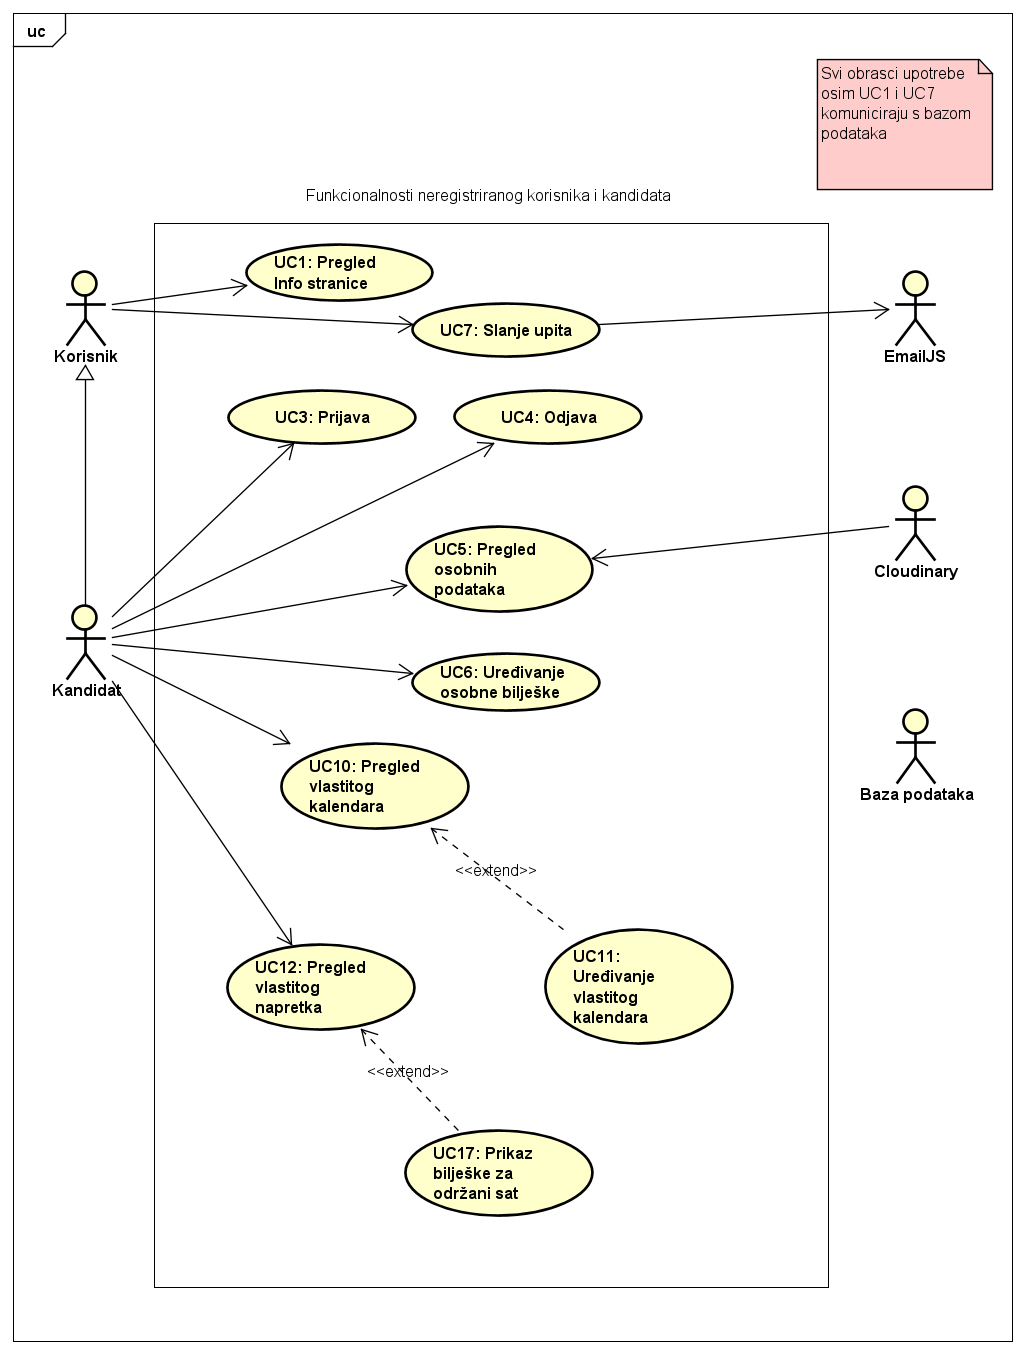
\includegraphics[width=\textwidth]{slike/UseCase Diagram3.png}
		\centering
		\vspace{-1cm}
		\caption{Dijagram obrazaca uporabe, funkcionalnost korisnika i Kandidata}
		\label{fig:promjene}
	\end{figure}

  \begin{figure}[H]
		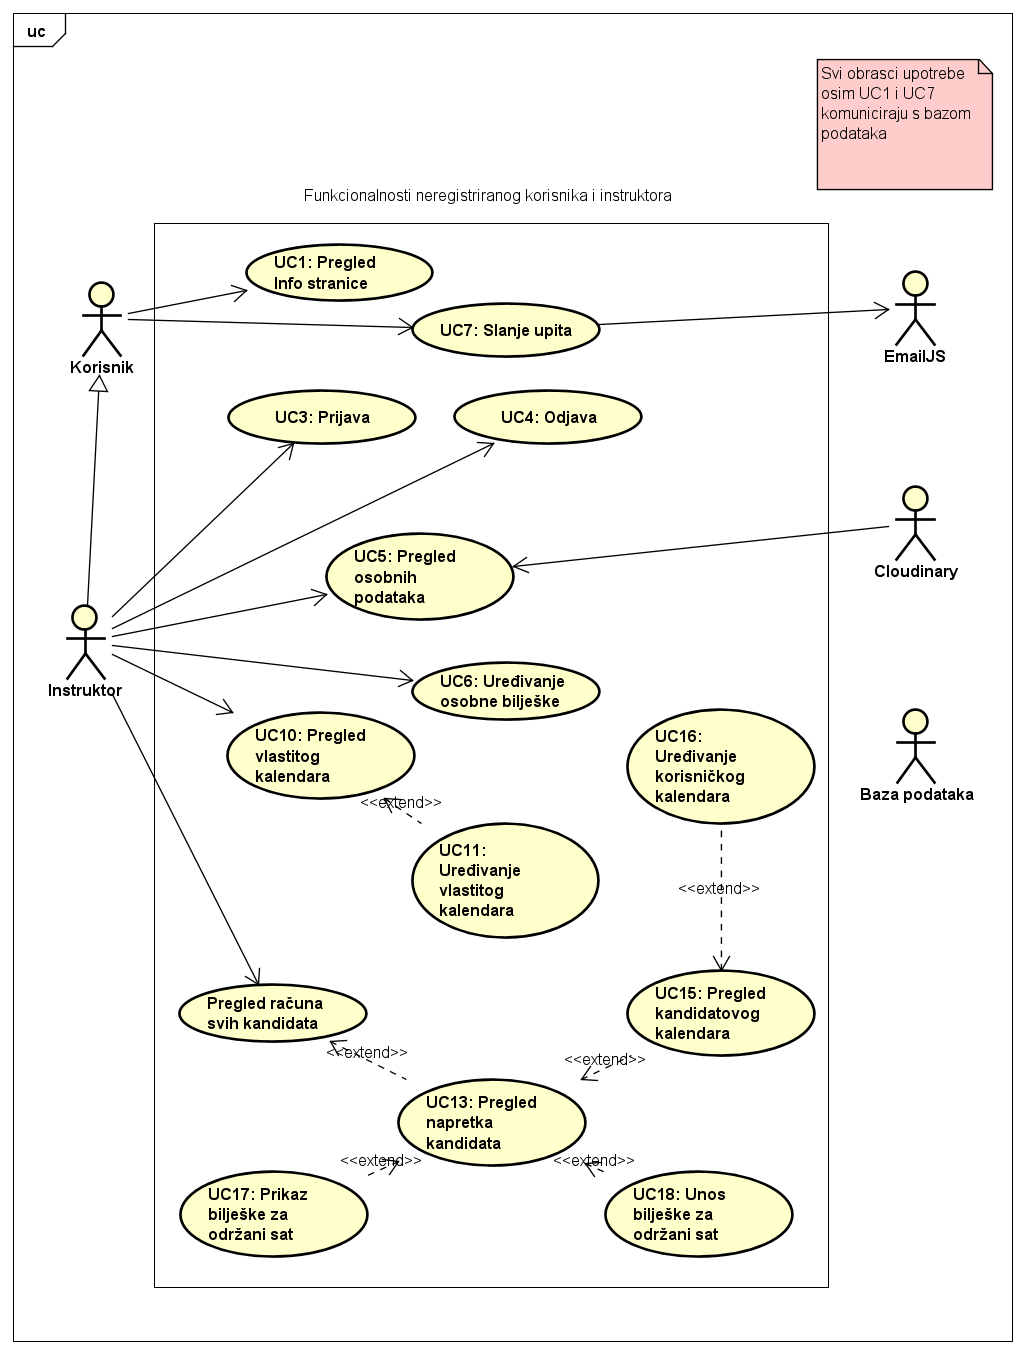
\includegraphics[width=\textwidth]{slike/UseCase Diagram2.png}
		\centering
		\vspace{-1cm}
		\caption{Dijagram obrazaca uporabe, funkcionalnost korisnika i Instruktora}
		\label{fig:promjene}
	\end{figure}

  \begin{figure}[H]
		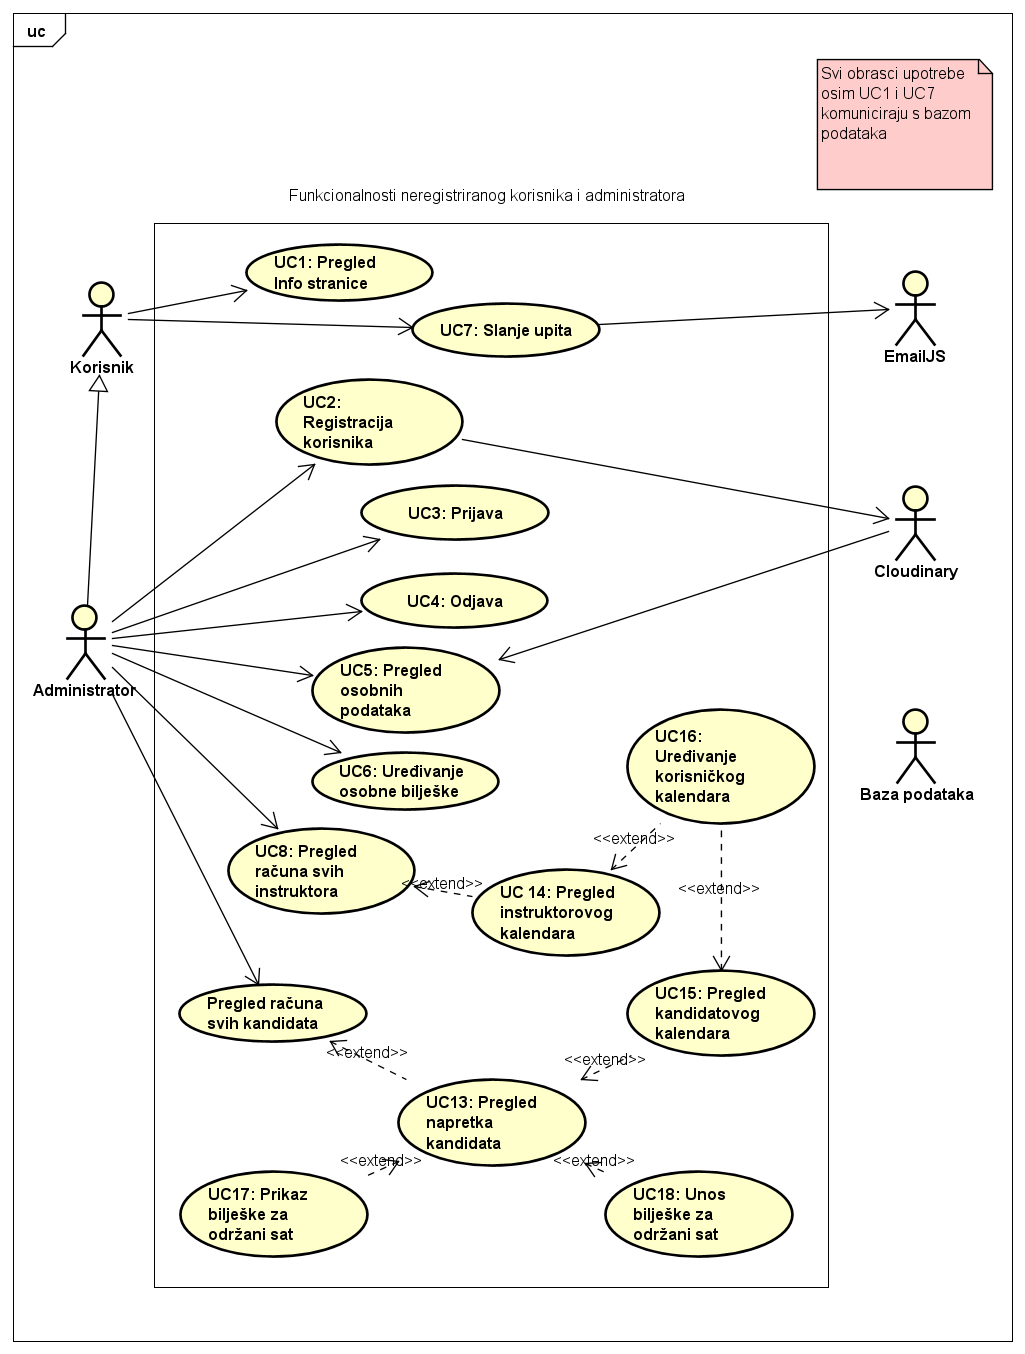
\includegraphics[width=\textwidth]{slike/UseCase Diagram1.png}
		\centering
		\vspace{-1cm}
		\caption{Dijagram obrazaca uporabe, funkcionalnost korisnika i Administratora}
		\label{fig:promjene}
	\end{figure}

 







    \chapter{Baza podataka}


  
\section{ER model}

Za konceptualno modeliranje baze podataka najprije je definiran entitetsko-relacijski model koji pomoću entiteta predstavlja objekte u stvarnom svijetu. Svaki entitet opisan je svojim atributima. Posebno se definira ključni atribut koji definira svojstvo koje identificira entitet. Relacije opisuju kako su entiteti međusobno povezani. Na slici 2.1. možemo vidjeti grafički prikaz ER modela. Svaki entitet prikazan je pravokutnikom, a njegovi atributi elipsama. Relacije su prikazane rombovima, a same veze linijama. Baza podataka ima sljedeće entitete


\begin{packed_item}
			\item Uloga
                \item Korisnik
                \item Slika
			\item Bilješka
			\item Teren
			\item SatiVožnje
			\item Dogadjaj
		\end{packed_item}

\noindent Svaki od prethodno  navedenih entiteta zadovoljava prvu, drugu i treću normalnu formu. Prva normalna forma zahtjeva da svi atributi sadrže nedjeljive vrijednosti i da svaki atribut ima jedinstveni identifikator. Druga normalna forma zahtjeva da svi neključni atributi zavise od cijelog primarnog ključa, ne samo jednog njegovog dijela. Na kraju, treća normalna forma zahtjeva nepostojanje tranzitivne zavisnosti, tj. zahtijeva da neključni atributi ne zavise od drugih neključnih atributa.



\begin{figure}[H]
					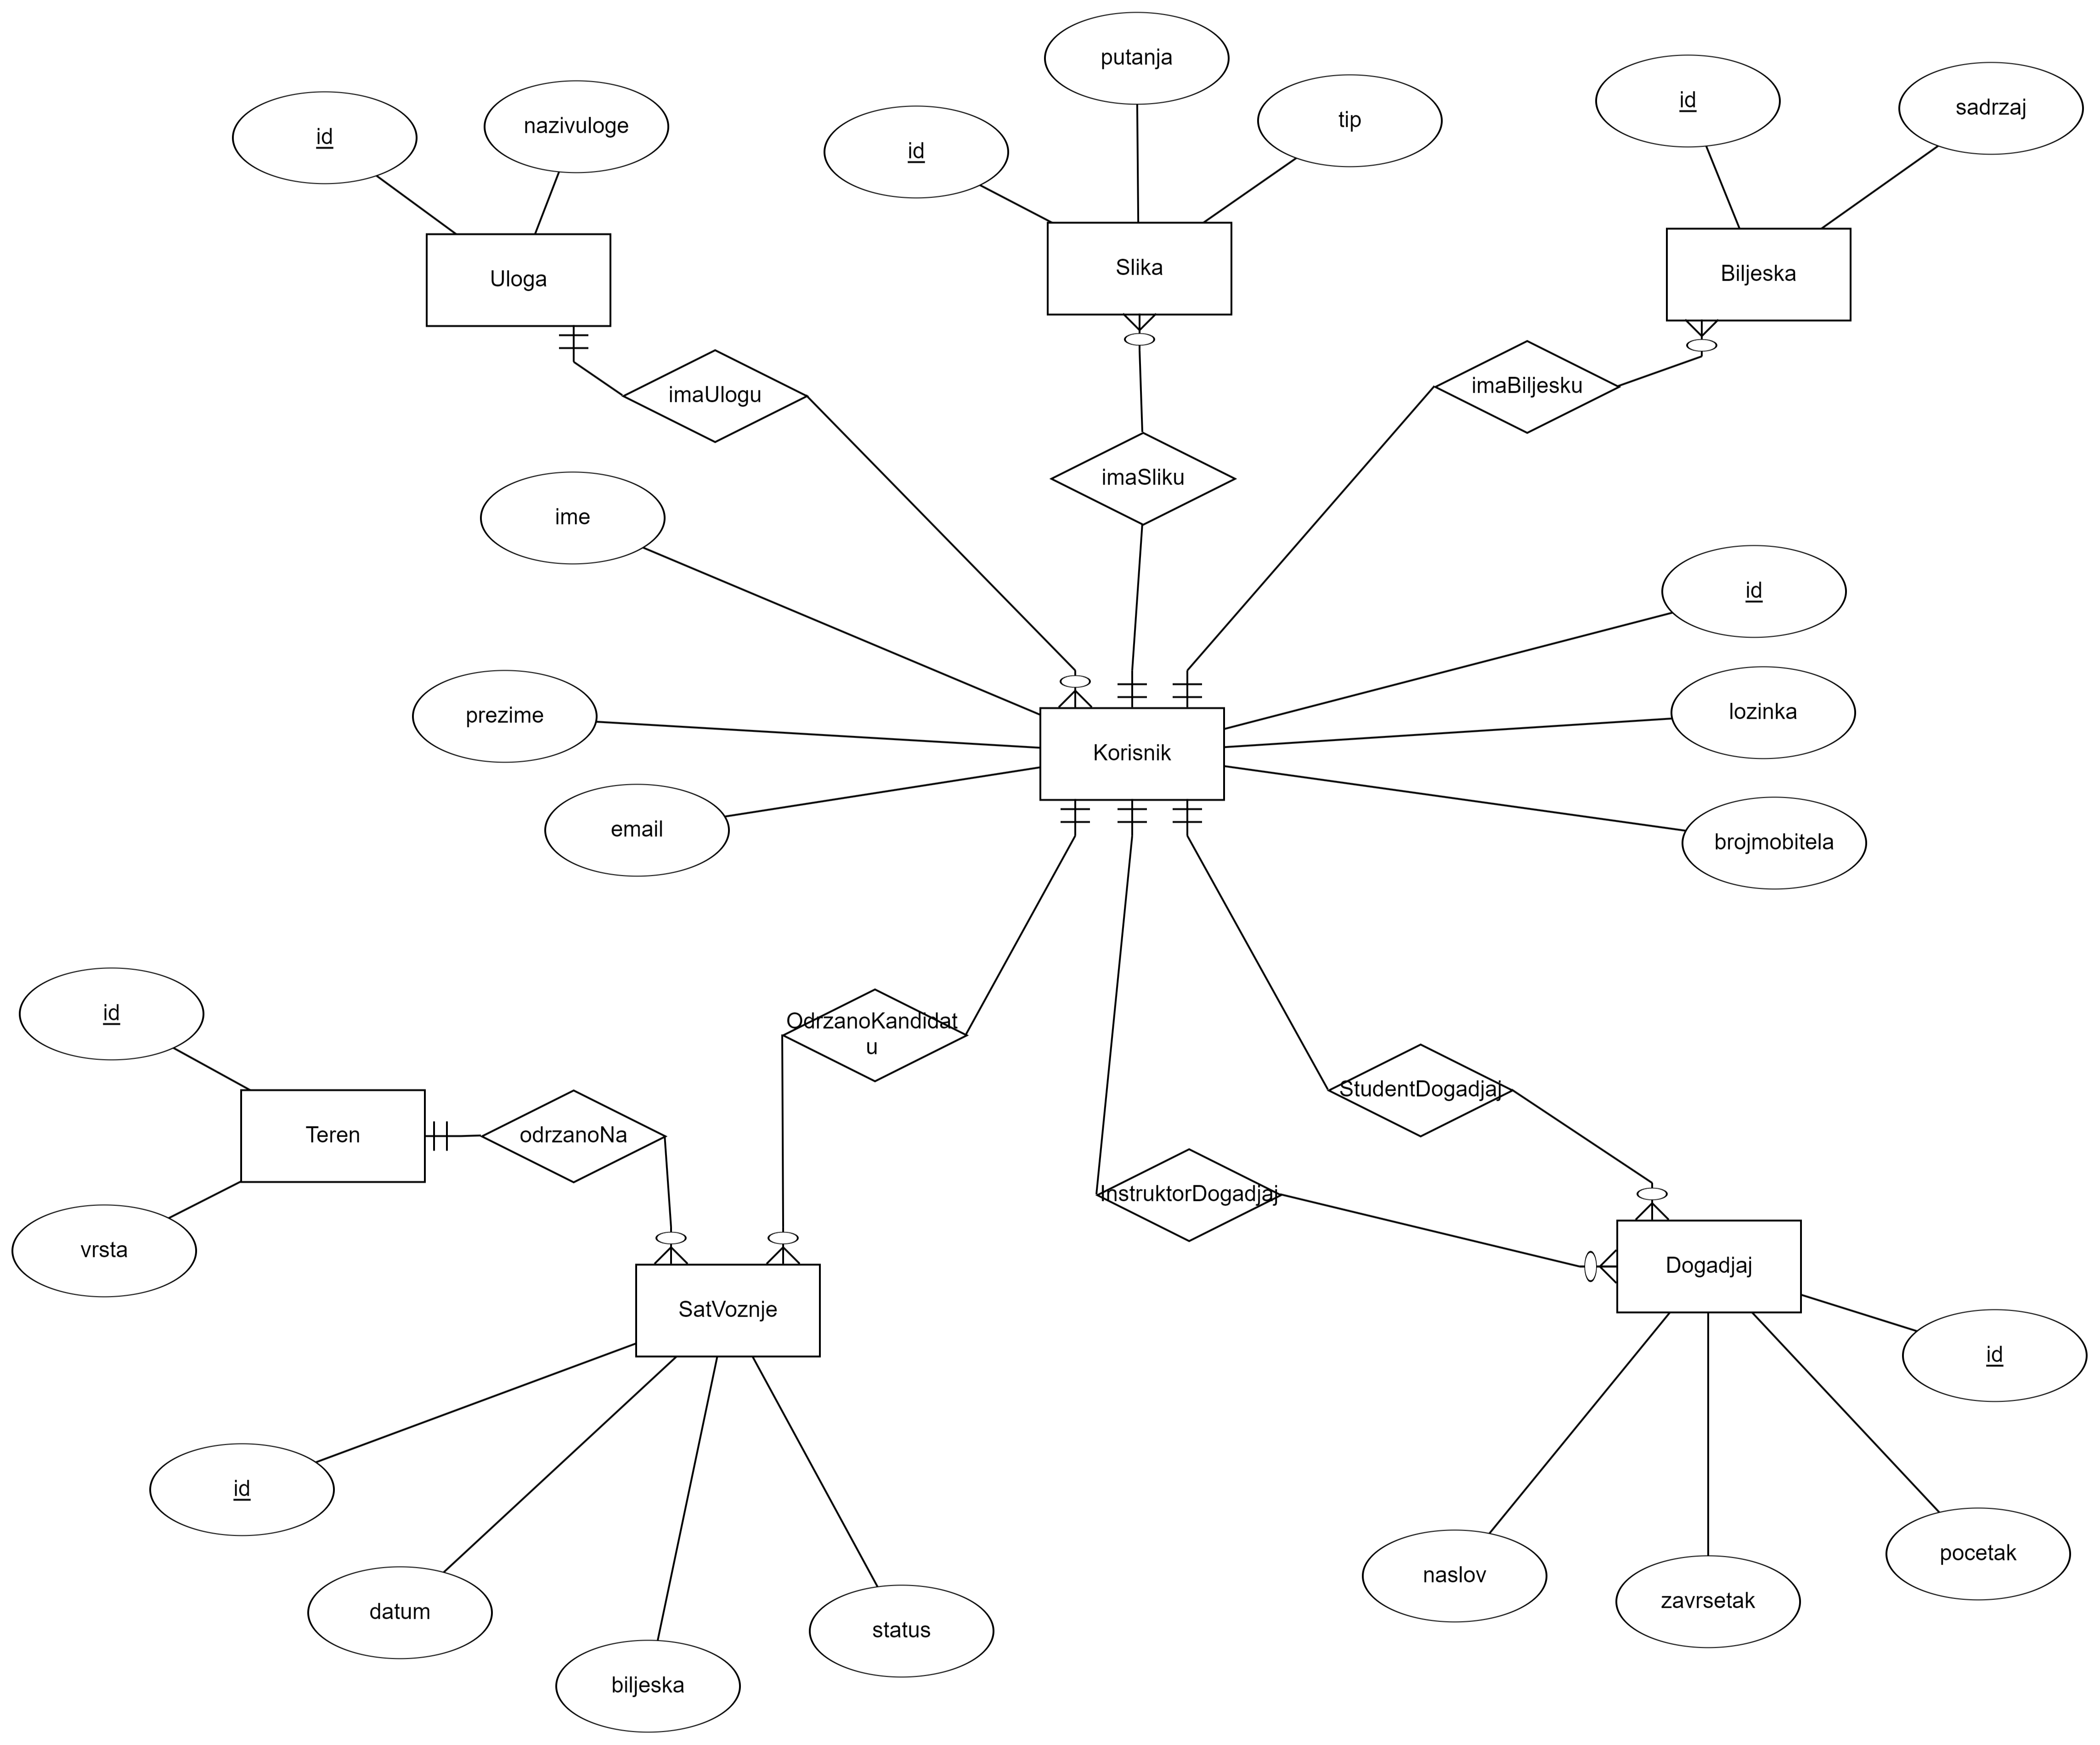
\includegraphics[width=\textwidth]{slike/ERBaza.png} 
					\centering
					\caption{ER dijagram baze podataka}
					\label{fig:promjene}
				\end{figure}




\noindent Svaki korisnik ima jedinstvenu ulogu, sliku i bilješku koja se odnosi samo na njega. Unos bilješke i slike za pojedinog korisnika nije obavezan, ali svaki registriran korisnik mora imati dodijeljenu ulogu. Sat vožnje može se održati na jednoj vrsti terena, dok se teren može povezati s više satova. Svakom korisniku može se održati više sati vožnje, ali jedan zapis vožnje odnosi se samo na jednog korisnika, odnosno kandidata. Događaj je povezan s korisnikom tako da se odnosi na minimalno jednog, a maksimalno dva korisnika. Postoje događaji koji se odnose samo na instruktora ili samo na kandidata, primjerice raspoloživost kandidata za održavanje obuke, dok sam termin održavanja obuke se odnosi i na kandidata i na instruktora. 


\section{Opis relacija}




 
 \noindent Entitet \textbf{Uloga}  sadrži informaciju o ulozi korisnika u sustavu. Svi atributi moraju biti definirani i unose se za svakog korisnika.

\label{tab:uloga}
\begin{longtblr}[
    label=none,
    entry=none
]{
    width = \textwidth,
    colspec = {|X[8,l]|X[6,l]|X[20,l]|},
    rowhead = 1
}
\hline 
\SetCell[c=3]{c}{\textbf{Uloga}} \\ \hline[3pt]
\SetCell{LightGreen}
ulogaID & BIGINT & jedinstveni identifikator uloge \\ \hline
nazivuloge & VARCHAR & opis korisničke uloge \\ \hline
\end{longtblr}



\noindent Entitet \textbf{Korisnik} sadrži korisničke podatke o svakom korisniku u sustavu. Svi atributi moraju biti definirani budući da entitet sadrži sve relevantne informacije o registriranom korisniku aplikacije.



\label{tab:korisnik}
\begin{longtblr}[
    label=none,
    entry=none
]{
    width = \textwidth,
    colspec = {|X[8,l]|X[6,l]|X[20,l]|},
    rowhead = 1
}
\hline 
\SetCell[c=3]{c}{\textbf{Korisnik}} \\ \hline[3pt]
\SetCell{LightGreen}
korisnikID & BIGINT & jedinstveni identifikator korisnika \\ \hline
ime & VARCHAR & ime korisnika \\ \hline
prezime & VARCHAR & prezime korisnika\\ \hline
email & VARCHAR & adresa elektroničke pošte \\ \hline
lozinka & VARCHAR & lozinka korisničkog računa \\ \hline
brojmobitela & VARCHAR & broj mobitela korisnika \\ \hline
\SetCell{LightBlue}ulogaID & BIGINT & jedinstveni identifikator uloge korisnika \\ \hline
\end{longtblr}



\noindent Entitet \textbf{Biljeska}  sadrži informaciju o bilješci za određenog korisnika u sustavu. Svi atributi moraju biti definirani i: obavezan unos za svakog korisnika.



\label{tab:biljeska}
\begin{longtblr}[
    label=none,
    entry=none
]{
    width = \textwidth,
    colspec = {|X[8,l]|X[6,l]|X[20,l]|},
    rowhead = 1
}
\hline 
\SetCell[c=3]{c}{\textbf{Bilješka}} \\ \hline[3pt]
\SetCell{LightGreen}
biljeskaID & BIGINT & jedinstveni identifikator bilješke \\ \hline
sadrzaj & VARCHAR & tekstualni zapis bilješke \\ \hline
\SetCell{LightBlue}korisnikID & BIGINT & jedinstveni identifikator korisnika \\ \hline
\end{longtblr}



\noindent Entitet \textbf{Slika}  sadrži putanju do slike određenog korisnika u sustavu. Svi atributi moraju biti definirani: obavezan unos za svakog korisnika.


\label{tab:slika}
\begin{longtblr}[
    label=none,
    entry=none
]{
    width = \textwidth,
    colspec = {|X[8,l]|X[6,l]|X[20,l]|},
    rowhead = 1
}
\hline 
\SetCell[c=3]{c}{\textbf{Slika}} \\ \hline[3pt]
\SetCell{LightGreen}
slikaID & BIGINT & jedinstveni identifikator zapisa \\ \hline
tip & VARCHAR & tip medijskog sadržaja (image) \\ \hline
putanja & VARCHAR & putanja do slike \\ \hline
\SetCell{LightBlue}korisnikID & BIGINT & jedinstveni identifikator korisnika  \\ \hline
\end{longtblr}




\noindent Entitet \textbf{Teren} sadrži informaciju o vrsti terena na kojoj je održan sat vožnje. Moguće vrijednosti su "V" - vježbalište koje označava održavanje sata na poligonu  i "C" - cesta koja označava održavanje sata na otvorenoj cesti. Svi atributi moraju biti definirani.


\label{tab:teren}
\begin{longtblr}[
    label=none,
    entry=none
]{
    width = \textwidth,
    colspec = {|X[8,l]|X[6,l]|X[20,l]|},
    rowhead = 1
}
\hline 
\SetCell[c=3]{c}{\textbf{Teren}} \\ \hline[3pt]
\SetCell{LightGreen}
terenID & BIGINT & jedinstveni identifikator terena \\ \hline
vrsta & VARCHAR & vrsta terena \\ \hline
\end{longtblr}





\noindent Entitet \textbf{SatVoznje} sadrži informaciju o održanom satu vožnje uključujući polaznika autoškole i teren na kojem je održan sat vožnje. Navedeni atributi predstavljaju zapravo strane ključeve. Svi atributi moraju biti definirani.

\label{tab:satvoznje}
\begin{longtblr}[
    label=none,
    entry=none
]{
    width = \textwidth,
    colspec = {|X[8,l]|X[6,l]|X[20,l]|},
    rowhead = 1
}
\hline 
\SetCell[c=3]{c}{\textbf{SatVoznje}} \\ \hline[3pt]
\SetCell{LightGreen}
satID & BIGINT & jedinstveni identifikator održanog sata \\ \hline
datum & DATE & datum održanog sata\\ \hline
biljeska & VARCHAR & komentar od strane instruktora \\ \hline
status & VARCHAR & status \\ \hline
\SetCell{LightBlue}kandidatID & BIGINT & jedinstveni identifikator kandidata kojem je održan sat obuke \\ \hline
\SetCell{LightBlue}terenID & BIGINT & jedinstveni identifikator terena na kojem je održan sat \\ \hline
\end{longtblr}



\noindent Entitet \textbf{Dogadjaj}  sadrži informaciju o pojedinom zapisu u kalendaru kandidata i instruktora. Jedinstveni identifikatori kandidata i instruktora su strani ključevi. Budući da svaki korisnik može sam unositi događaje u svoj kalendar, te instruktor može kandidatu zakazati sat, određeni zapisi mogu imati oba strana ključa definirana, dok je dozvoljeno izostavljanje jednog od ključeva ovisno u korisniku koji unosi događaj

\begin{longtblr}[
    label=none,
    entry=none
]{
    width = \textwidth,
    colspec = {|X[8,l]|X[6,l]|X[20,l]|},
    rowhead = 1
}
\hline 
\SetCell[c=3]{c}{\textbf{Dogadjaj}} \\ \hline[3pt]
\SetCell{LightGreen}
dogadjajID & BIGINT & jedinstveni identifikator događaja \\ \hline
pocetak & TIMESTAMP & datum održanog sata\\ \hline
zavrsetak & TIMESTAMP & naziv terena \\ \hline
naslov & VARCHAR & naslov događanja\\ \hline
\SetCell{LightBlue}kandidatID & BIGINT & jedinstveni identifikator kandidata  \\ \hline
\SetCell{LightBlue}instruktorID & BIGINT & jedinstveni identifikator instruktora \\ \hline


\end{longtblr}


\section{Relacijski model}


     
Na slici 3.1. možemo vidjeti relacijsku shemu baze podataka. 
\begin{figure}[H]
					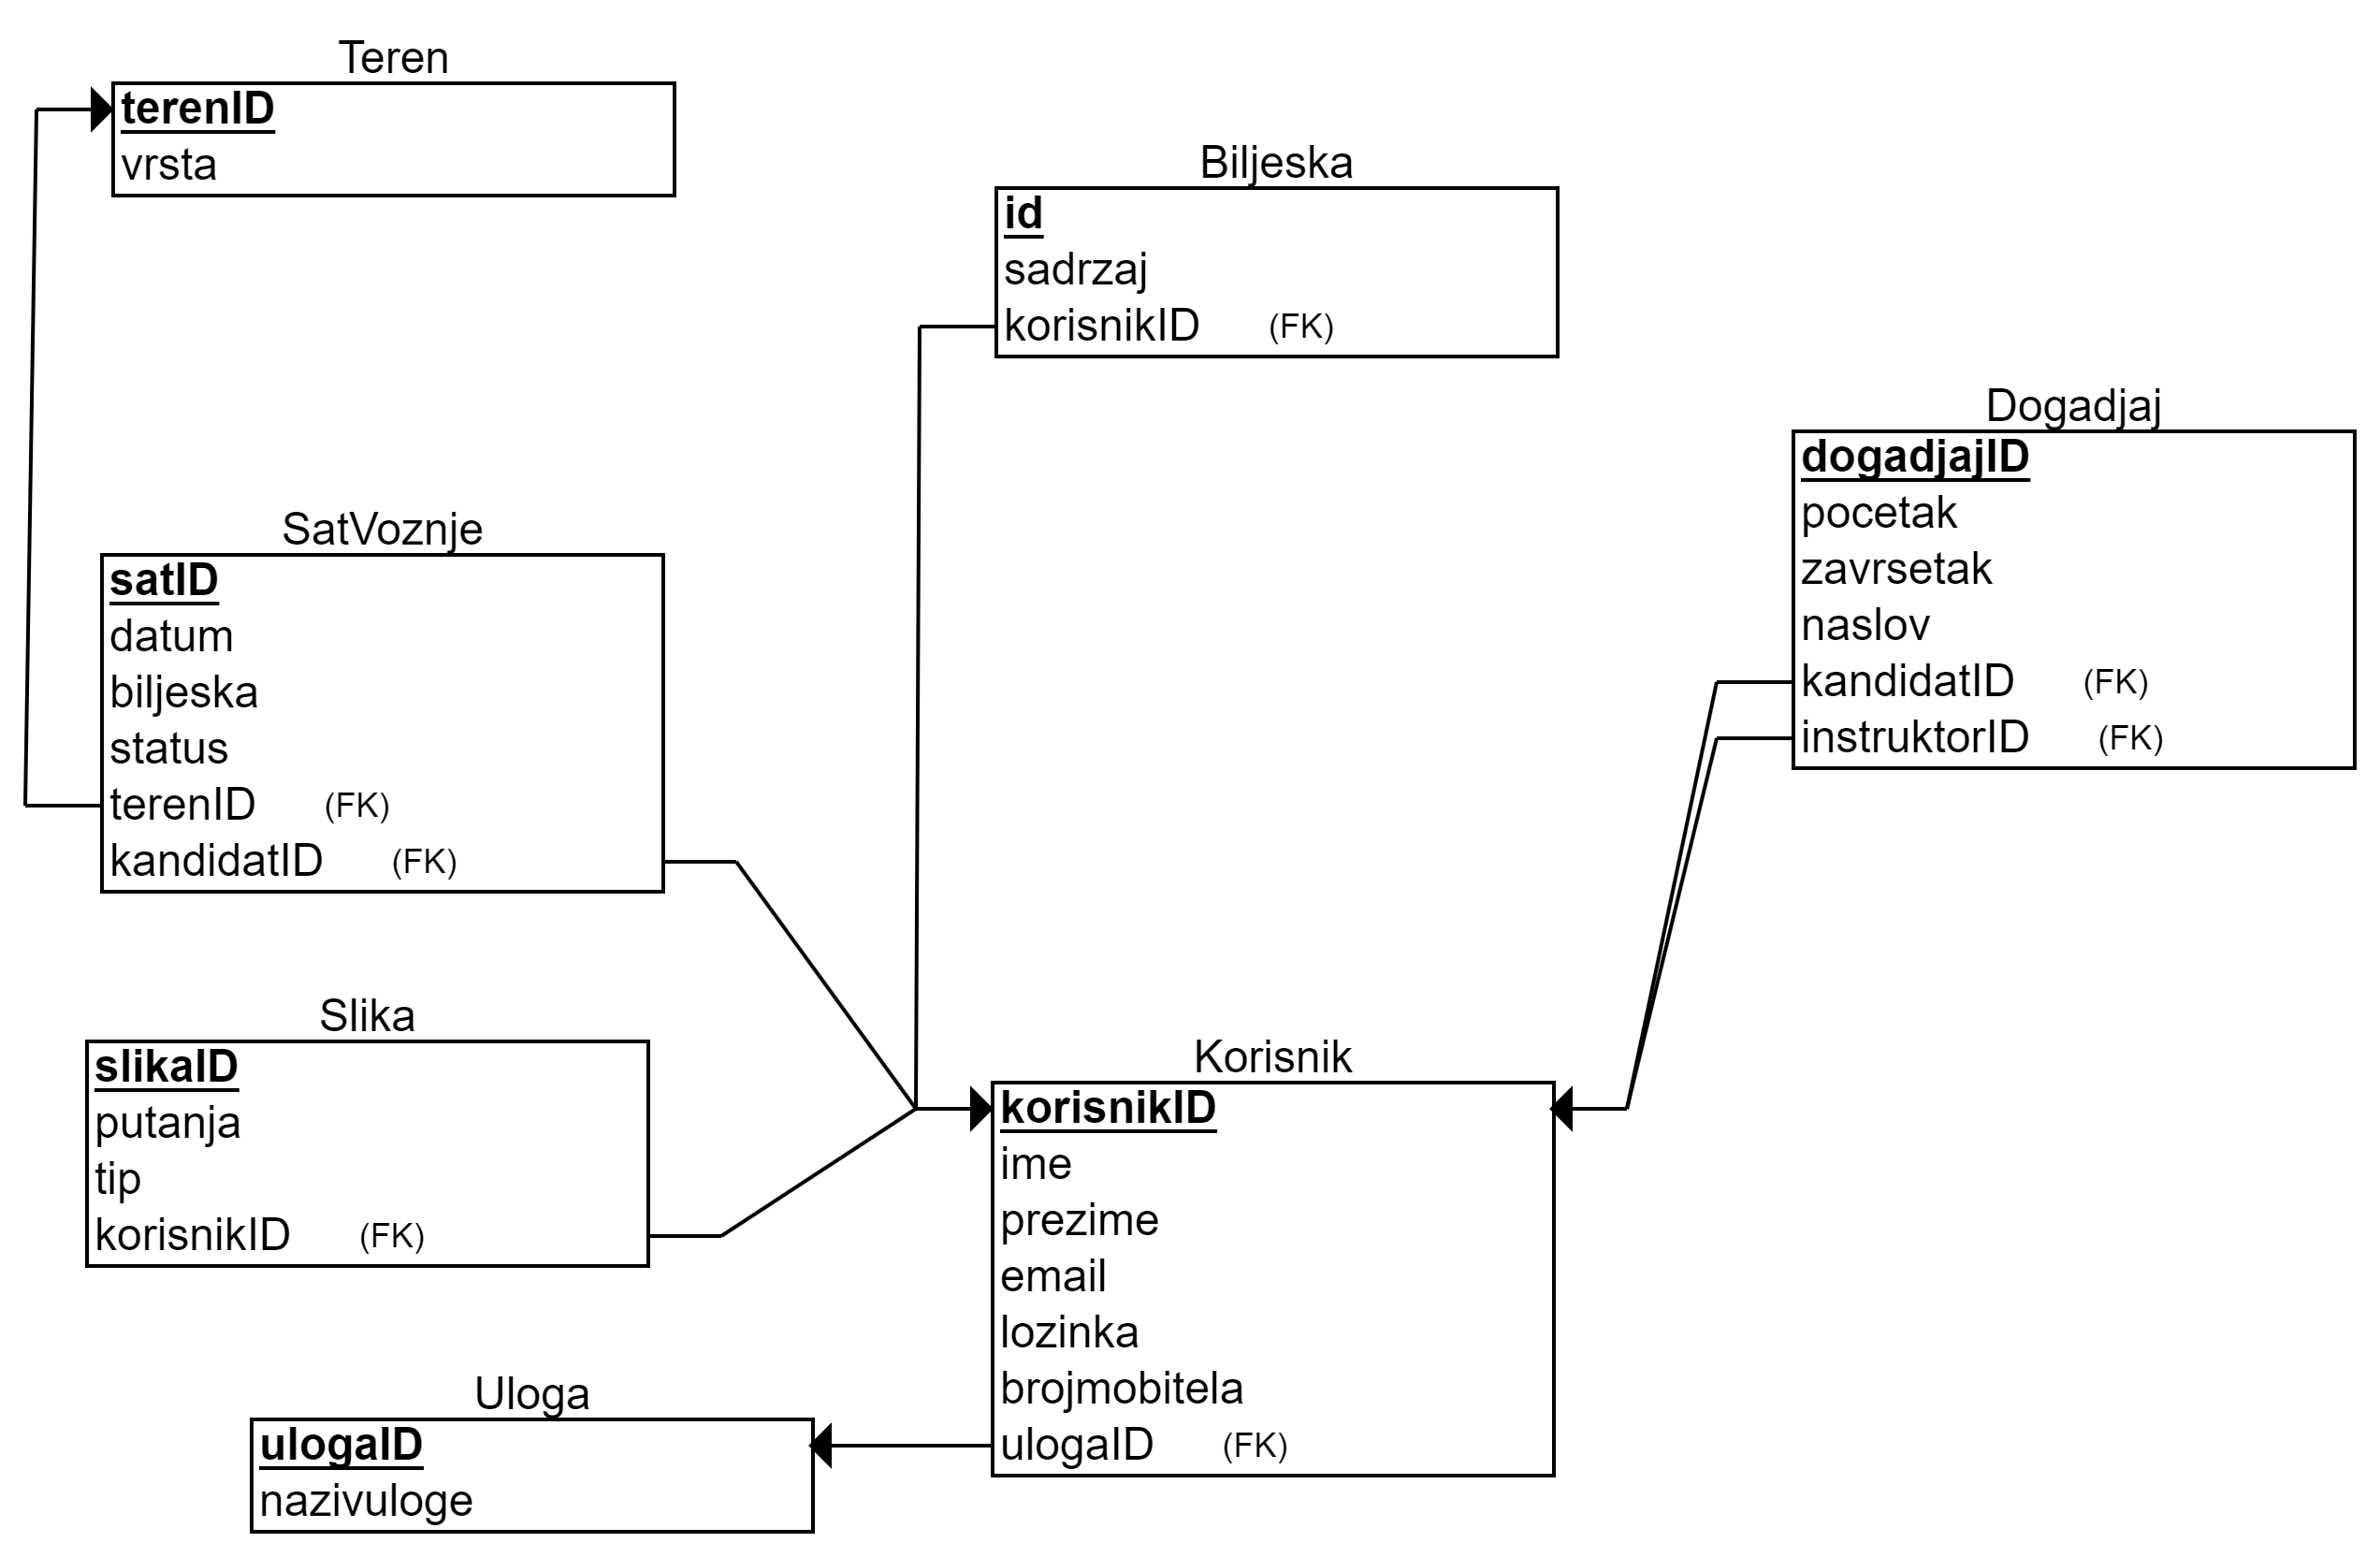
\includegraphics[width=\textwidth]{slike/RelBaza.png} 
					\centering
					\caption{Dijagram baze podataka}
					\label{fig:promjene}
				\end{figure}


\noindent Sustav koristi H2 relacijsku bazu podataka koja se posebno ističe po lakoj integraciji s aplikacijama razvijenim u programskom jeziku Java. Glavna karakteristika aplikacije je njena brzina i učinkovitost zbog organizacije i pohrane podataka u radnu memoriju, dok se inače u sustavima za upravljanje podacima koriste mehanizmi za pohranu na disku. Kao takva, H2 baza pruža podršku standardnim SQL naredbama. Razvoj i testiranje same baze posebno olakšava i grafičko korisničko sučelje kojem se pristupa putem weba. Iako je H2 odličan izbor za razvojne faze projekta, koristit će se i u proizvodnom okruženju web aplikacije zbog manjih zahtjeva na bazu podataka. Budući da u sustavu postoje samo tri uloge korisnika, zbog jednostavnosti u implementaciji su združeni entiteti \noindent \textbf{Korisnik} i \noindent \textbf{Uloga}. Iz istog razloga združeni su i entiteti \noindent \textbf{Teren} i \noindent \textbf{SatVoznje}. U konačnici, implementacija aplikacije je realizirana pomoću pet entiteta: \noindent \textbf{Korisnik}, \noindent 
    \textbf{Slika},  \noindent
     \textbf{Bilješka}, \noindent \textbf{SatVožnje}, \noindent \textbf{Dogadjaj}.





    \chapter{Implementacija}
\section{Korištene tehnologije}

\subsection{Spring Boot}
Za razvoj backenda web aplikacije "Vožnja +" izabran je Spring Boot razvojni okvir koji znatno pojednostavljuje i olakšava razvoj aplikacija u Programskom jeziku Java. Glavna prednost Spring Boota je smanjena konfiguracijska složenost i ubrzan razvoj aplikacije. Razvoj aplikacije započeo je upotrebom Spring inicijalizatora projekta na kojem se odabire projekt (Maven), programski jezik (Java) i verzija Spring Boota. Pri inicijalizaciji dodaju se potrebne ovisnosti koje se kasnije po potrebi nadograđuju u pom.xml datoteci. Osnovne konfiguracijske postavke definiraju se u datoteci application.properties.  U razvoju aplikacije ključnu ulogu igraju anotacije koje omogućuju konfiguraciju i upravljanje komponentama bez potrebne za opsežnim XML konfiguracijama. Primjerice, anotacija @Autowired koristi se za automatsku injekciju zavisnosti koja eliminira potrebu za ručnom konfiguracijom. To znači da umjesto ručnog konfiguriranja komponente pri svakom njenom korištenju, sve što trebamo napraviti je iznad instanciranja komponente dodati spomenutu anotaciju. Ostatak anotacija bit će objašnjeni u poglavlju "Poslužitelj" gdje će se detaljnije objasniti  implementacija poslužiteljske strane i korištenje karakterističnih Spring Boot anotacija. Korišteni radni okvir je IntelliJ.
\subsection{React}
Za razvoj frontenda korišten je skriptni jezik JavaScript koji se izvršava u web pregledniku korisnika web aplikacije. Za razvoj korisničkih sučelja korištena je Raect razvojna biblioteka. React je biblioteka otvorenog koda temeljena na komponentama koje se koriste s izgradnju sučelja. Svaka komponenta ima mogućnost održavanja svog stanja i komponiranja u složenije dijelove grafičkog sučelja. Glavna karakteristika Reacta je njegov dizajn koji omogućava ponovno renderiranje komponente tek pri promjeni podataka što je učinkovitije nego ponovno renderiranje cijele stranice. Pored Reacta, za učinkovit razvoj korisničkih sučelja korištena je  Chakra UI biblioteka komponenti koja pruža polu-gotove gradivne blokove za izgradnju aplikacije. Svaki gradivni element prilagođen je svojoj namjerni kako bi se osiguralo što bolje korisničko iskustvo. Korišteni radni okvir je Visual Studio Code.

\subsection{Cloudinary}
Za skladištenje i manipulaciju medijskim sadržajem u aplikaciji korištena je Cloudinary platforma kojoj se pristupa pomoću API-ja (engl. application programming interface). Glavne funkcionalnosti Cloudinary platforme koje su korištene za aplikaciju su skladištenje i dohvat fotografija. Platforma osigurava sigurnost i podržava kontroliran pristup budući da se pri konfiguraciji servisa koriste Cloud name (ime oblaka), API key (API ključ) i API secret (API tajna) koji se provjeravaju pri svakom pristupu.

\subsection{EmailJS}
Integracija s Gmail servisom ostvarena je pomoću EmailJS servisa koji omogućava direktno slanje emailova iz JavaScript aplikacija bez potrebe za poslužiteljem. Na ovaj način omogućeno je učinkovito slanje mailova direktno iz aplikacije. Nakon konfiguracije, servis brine o komunikaciji i autentificiranom pristupu svojim uslugama.

\section{Dijagram razmještaja sustava}
Na slici 4.1. možemo vidjeti dijagram razmještaja sustava. Za arhitekturu odabrana je arhitektura poznata po nazivu "klijent-poslužitelj". Glavna karakteristika spomenute arhitekture je razdvojenog funkcionalnosti na usluge koje pruža poslužitelj i usluge koje pruža klijent. Korisnici web aplikacije pristupaju aplikaciji putem web preglednika na vlastitom računalu. Korisničko računalo ima ulogu klijenta koje u ime korisnika obavlja zahtjeve prema poslužitelju. Web poslužitelj i poslužitelj baze podataka nalaze se na zasebnom računalu. Interakcija između korisničkog i poslužiteljskog računala odvija se putem HTTP (HyperText Transfer Protocol) protokola. Osnovne karakteristike HTTP protokola su komunikacija putem zahtjeva i odgovora te neovisnost novog zahtjeva o prethodno poslanim zahtjevima. 

\begin{figure}[H]
					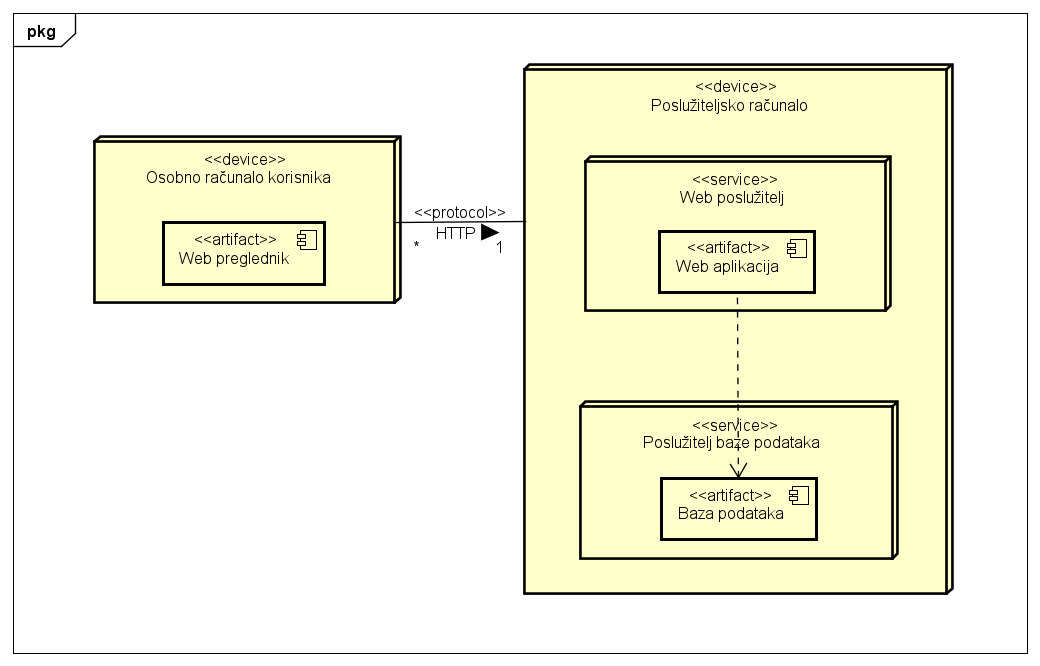
\includegraphics[width=\textwidth]{slike/DeploymentDiagram.png} 
					\centering
					\caption{Dijagram razmještaja sustava}
					\label{fig:promjene}
				\end{figure}
\subsection{Klijent}
Klijentska strana  zasnovana je na funkcijskim komponentama pomoću kojih se gradi izgled cijele aplikacije. React koristi virtualni DOM (engl. Data Object Model) za poboljšanje svojih performansi. Kada se stanje aplikacije promijeni, React prvo ažurira virtualni DOM koji onda uspoređuje s pravim modelom kako bi minimalno ažurirao stvarni model. App.js je ključna komponenta u kojoj su definirane korisničke rute i komponente koje se koriste za izgradnju pojedinih sučelja. Sučelje koje se prikazuje korisniku ovisi u njegovoj ulozi koja se sprema u memoriju sjednice. Svaka komponenta ima svoje unutarnje stanje koje određuje kako se komponenta prikazuje i ponaša. Za očuvanje stanja i ažuriranje komponenti koriste se dvije posebne funkcionalnosti Reacta: useState i useEffect hook-ovi. Hook-ovi služe za baratanje s popratnim efektima pojedine komponente. useState hook služi za održavanje lokalnog stanja funkcijskim komponentama, a useEffect hook služi za ažuriranje komponente, odnosno njenih podataka. Kako bi se moglo navigirati između različitih komponenti, korišten je React Router koji omogućava definiranje višestrukih ruta unutar aplikacije.

\subsection{Poslužitelj}
Aplikacija je izgrađena korištenjem objektno orijentirane paradigme i MVC (eng. Model-View-
Controller) arhitekturnog obrasca koji razdvaja prezentaciju podataka, njihov dohvat i manipulaciju. Implementacija poslužiteljske strane zasnovana je na reprezentacijskom prijenosu stanja, odnosno REST (Representational State Transfer) arhitekturalnom stilu čija glavna karakteristika manipulacija podacima korištenjem standardnih HTTP metoda kao što su GET, POST, PUT, i DELETE. Anotacija @Entity označava komponentu koja reprezentira informacije potrebne za rad aplikacije. Svaki entitet predstavlja podatke koji se prezentiraju kao tablica u bazi podataka. Korištenjem anotacije @Controller označena je kontrolerska komponenta koja je odgovorna za obradu zahtjeva koji dolaze od klijentske strane. Servisni sloj sadrži poslovnu logiku aplikacije te obavljaju sve potrebne operacije nad podacima. Servisi su zasebne komponente odvojene od kontrolera te se označavaju anotacijom @Service. Za podatkovni sloj zaduženo je standardizirano sučelje prema podacima pod nazivom JPA (Java Persistence API). Podatkovno sučelje naznačeno je anotacijom @Repository. 

\section{Sigurnost}
Za sigurnost sustava, odnosno implementaciju autentifikacije i autorizacije korisnika korišten je JSON Web Token (JWT). Korištenje tokena standardan je način sigurnog prijenosa podataka između dvaju partija, u ovom slučaju su to klijent i poslužitelj. Pri prijavi u sustav pomoću korisničkih podataka, korisnik, odnosno njegov web preglednik kao odgovor od poslužitelja dobiva izgeneriran token koji pohranjuje u sjednicu i koristi pri svakoj interakciji s poslužiteljem do kraja korištenja aplikacije. S druge strane, pri svakom zahtjevu poslužitelj iz tokena izvlači e-mail te provjerava postoji li korisnik u bazi te u skladu s provjerom obrađuje poslani zahtjev. Kako bi se spriječio neovlašten pristup određenim stranicama, pored autentifikacije putem JWT tokena, svakom korisniku u sustavu dodijeljena je uloga i u skladu s njom definirane korisničke ovlasti. Pri slanju zahtjeva klijent obavezno uključuje token u autorizacijsko zaglavlje svakog HTTP zahtjeva kako bi mogao pristupiti zaštićenim resursima.
    \chapter{Sučelja web aplikacije}
\noindent \textbf{Sučelja anonimnog korisnika}\\
\noindent Na slici 4.1. možemo vidjeti sučelje koje se prikazuje pri pokretanju aplikacije. Svakom anonimnom korisniku su u navigacijskoj traci omogućene opcije za povratak na početnu stranicu, prijavu u aplikaciju, pristup stranici s informacijama i pristup kontaktnoj formi. Klikom na gumb "Započnimo" korisnika se također preusmjerava na stranicu za prijavu
\begin{figure}[H]
					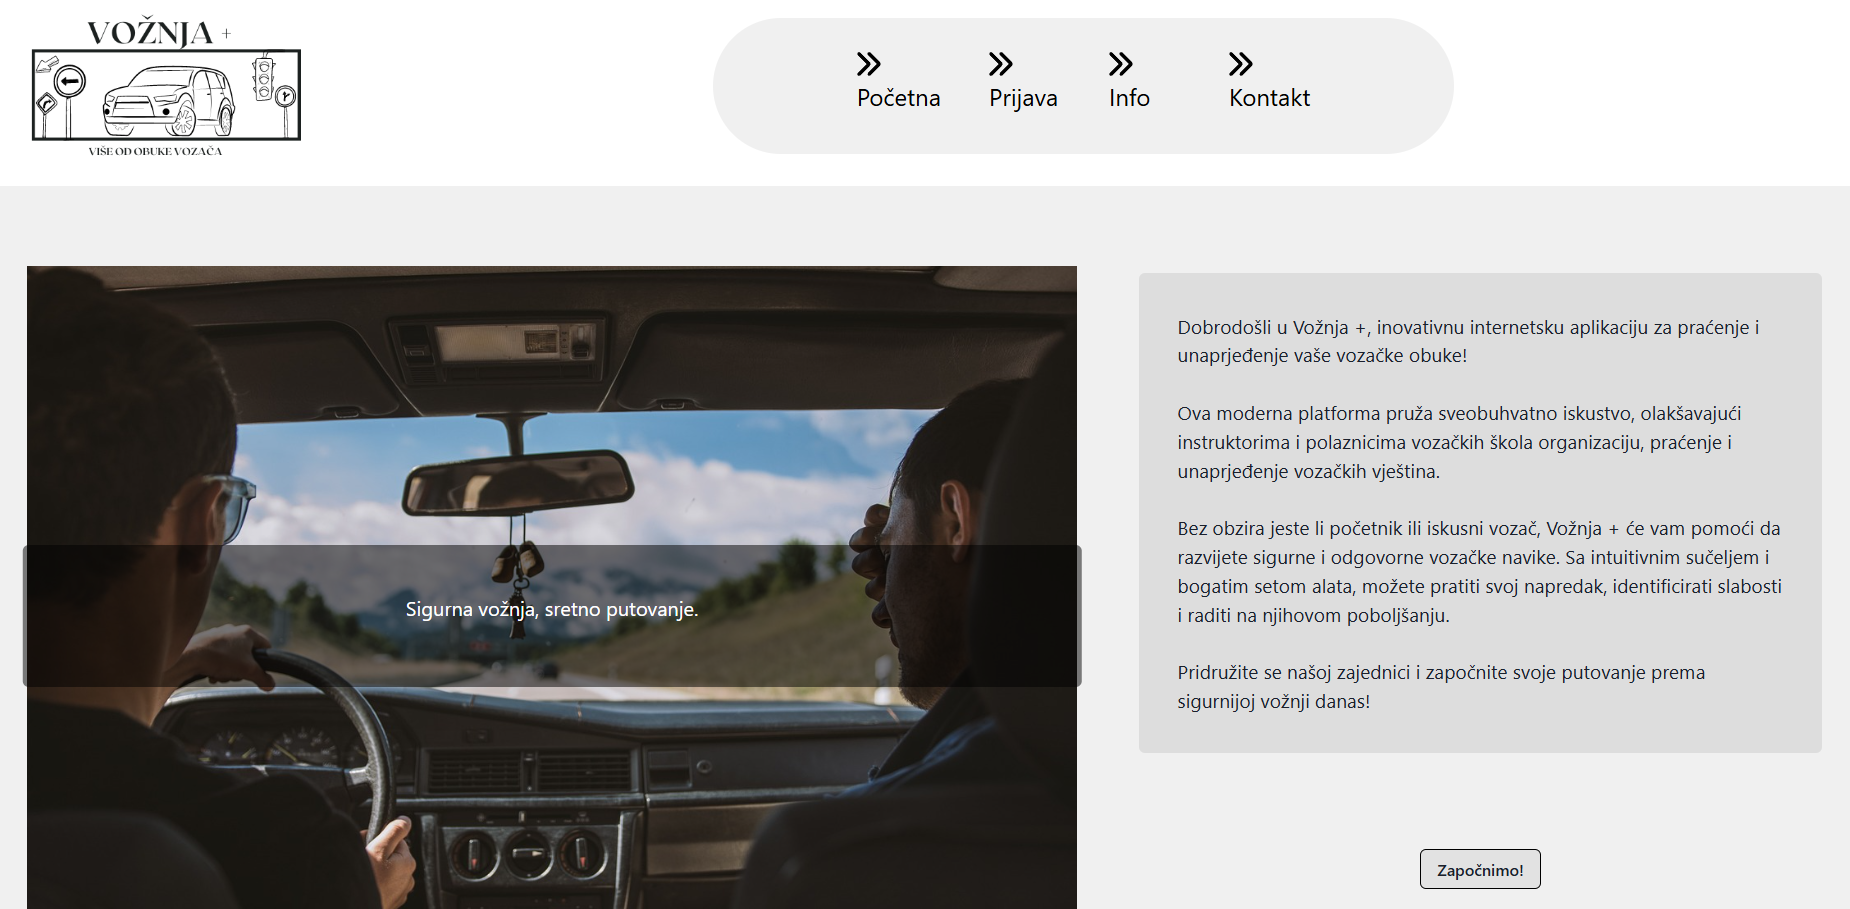
\includegraphics[width=\textwidth]{slike/anoniman1.png} 
					\centering
					\caption{Početna stranica}
					\label{fig:promjene}
				\end{figure}

\noindent Da bi se korisnik prijavio u sustav, u navigacijskoj traci odabire opciju za prijavu. Sučelje koje se prikazuje može se vidjeti na slici 4.2.

\begin{figure}[H]
					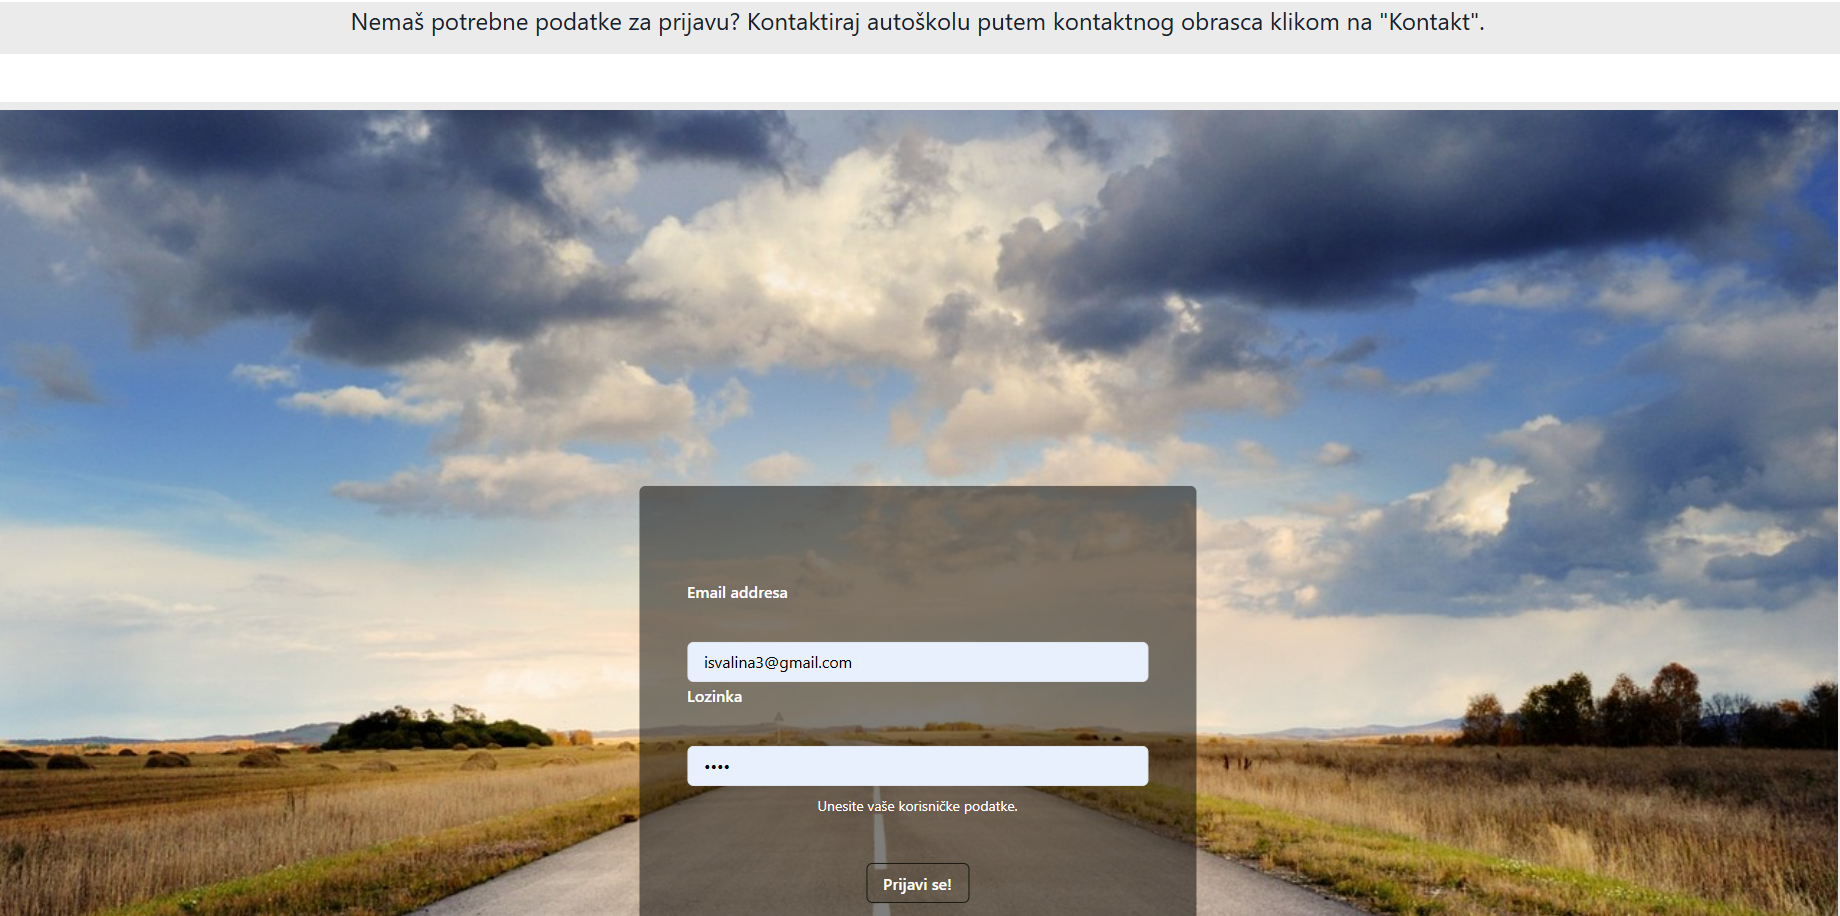
\includegraphics[width=\textwidth]{slike/anoniman2.png} 
					\centering
					\caption{Stranica za prijavu}
					\label{fig:promjene}
				\end{figure}

\noindent Ako korisnik želi dobiti više informacija o autoškoli i aplikaciji, može dabrati opciju "Info" u navigacijskoj traci. Sučelje koje mu se prikazuje je na slici 4.3. i 4.4.

\begin{figure}[H]
					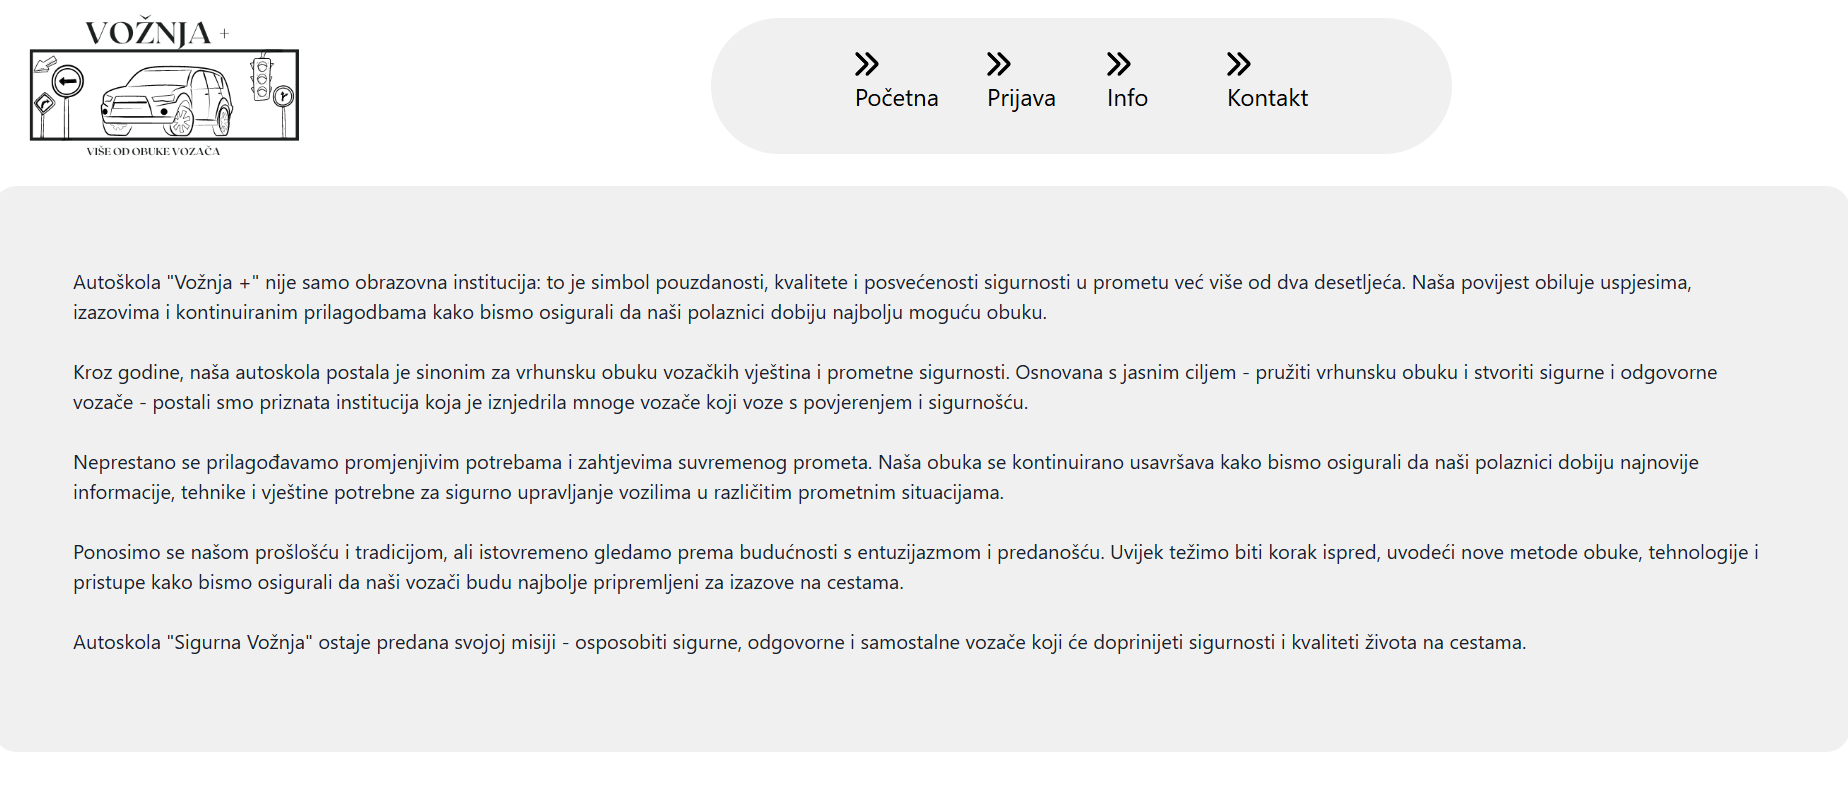
\includegraphics[width=\textwidth]{slike/anoniman3.png} 
					\centering
					\caption{Stranica s dodatnim informacijama}
					\label{fig:promjene}
				\end{figure}

    
\begin{figure}[H]
					
\includegraphics[width=\textwidth]{slike/anoniman4.png} 
					\centering
					\caption{Stranica s dodatnim informacijama}
					\label{fig:promjene}
				\end{figure}

\noindent Za slanje kontaktne forme korisnik odabire opciju "Kontakt" u navigacijskoj traci ili "Pošalji upit" te mu se prikazuje sučelje na slici 4.5.

\begin{figure}[H]
					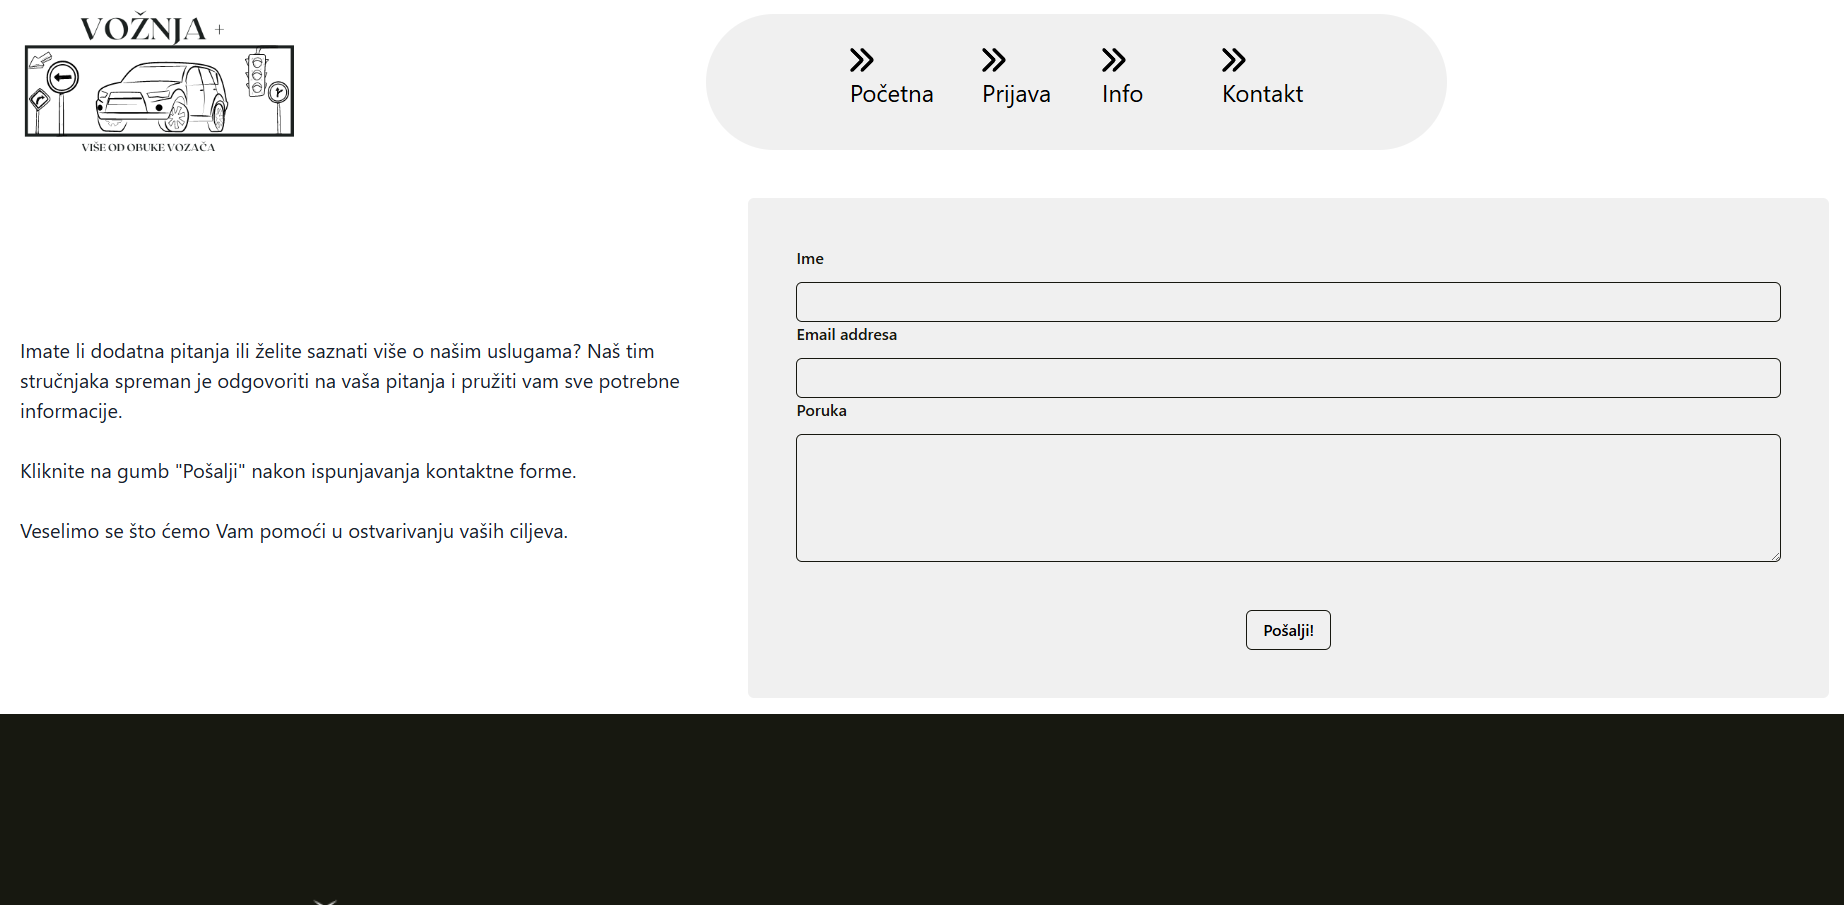
\includegraphics[width=\textwidth]{slike/anoniman5.png} 
					\centering
					\caption{Stranica s kontakt formom}
					\label{fig:promjene}
				\end{figure}


\noindent \textbf{Sučelja polaznika autoškole }\\

\noindent Nakon što se kandidat prijavi u aplikaciju, pored osnovnih, omogućen mu je pristup dodatnim web stranicama. Na slici 4.6. možemo vidjeti kako izgleda stranica s vlastitim korisničkim podacima kojoj može pristupiti svaki autentificiran korisnik.

\begin{figure}[H]
					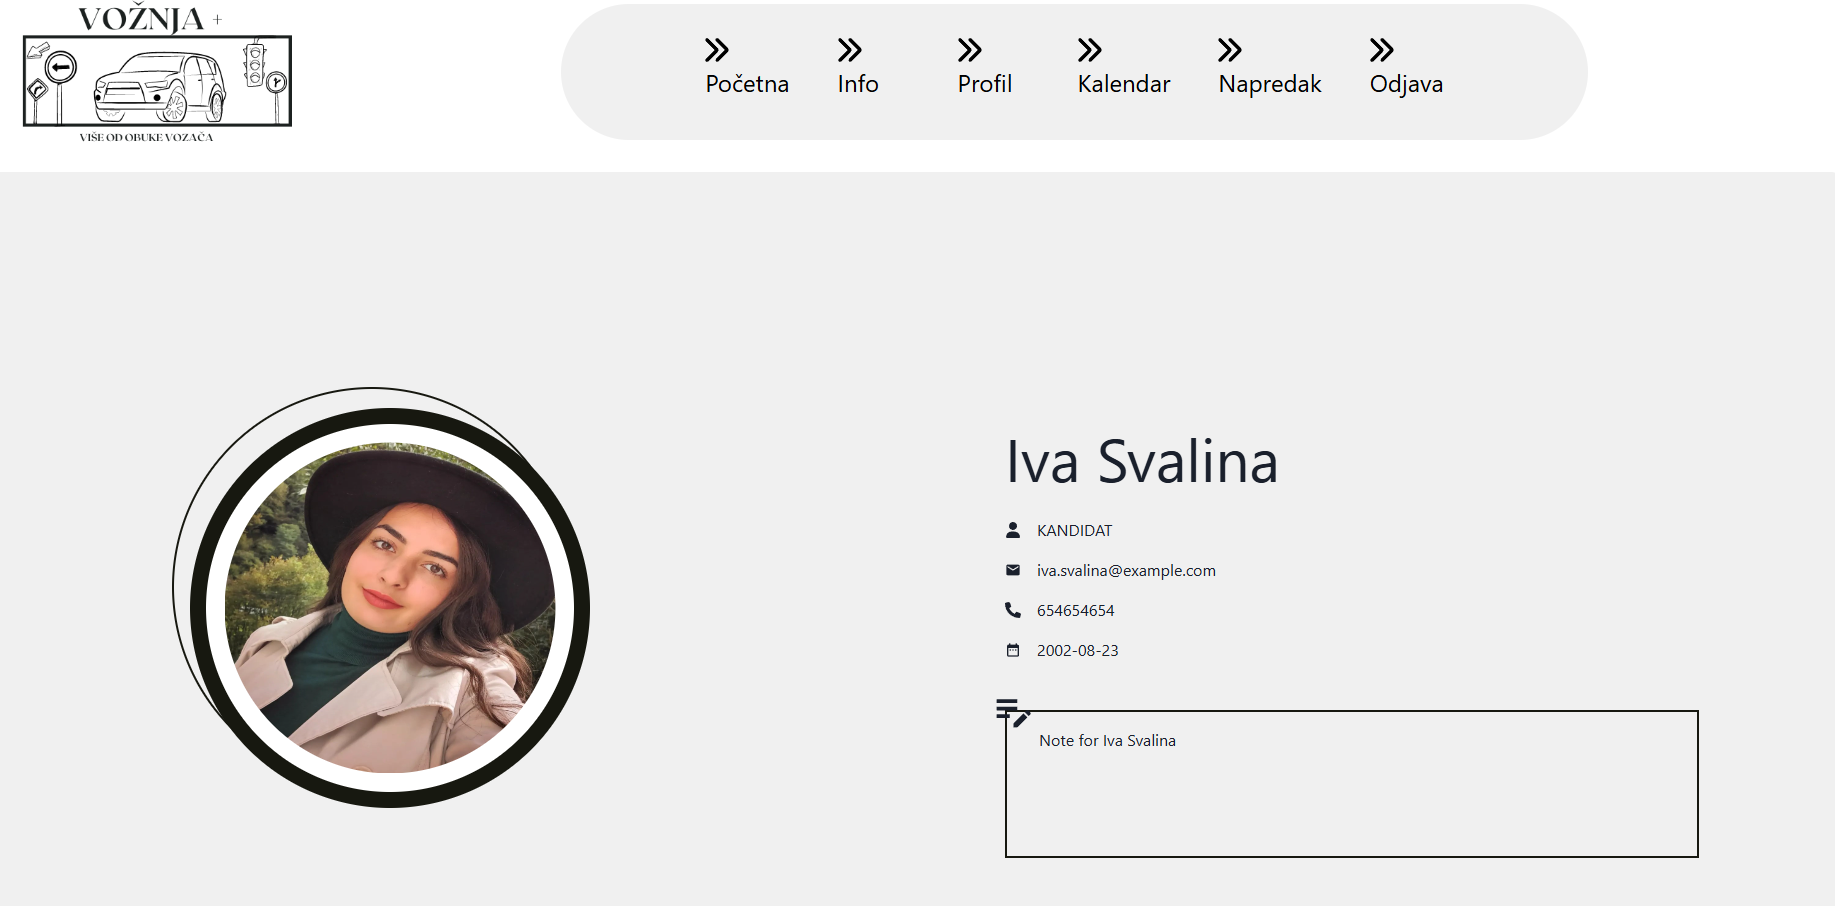
\includegraphics[width=\textwidth]{slike/kandidat1.png} 
					\centering
					\caption{Stranica s kontakt formom}
					\label{fig:promjene}
				\end{figure}

\noindent Odabirom opcija "Kalendar" u navigacijskoj traci korisniku se prikazuje sučelje na slici 4.7. Korisnik događaje u kalendaru može dodavati, uređivati i brisati, što je prikazano na slici 4.8.

\begin{figure}[H]
					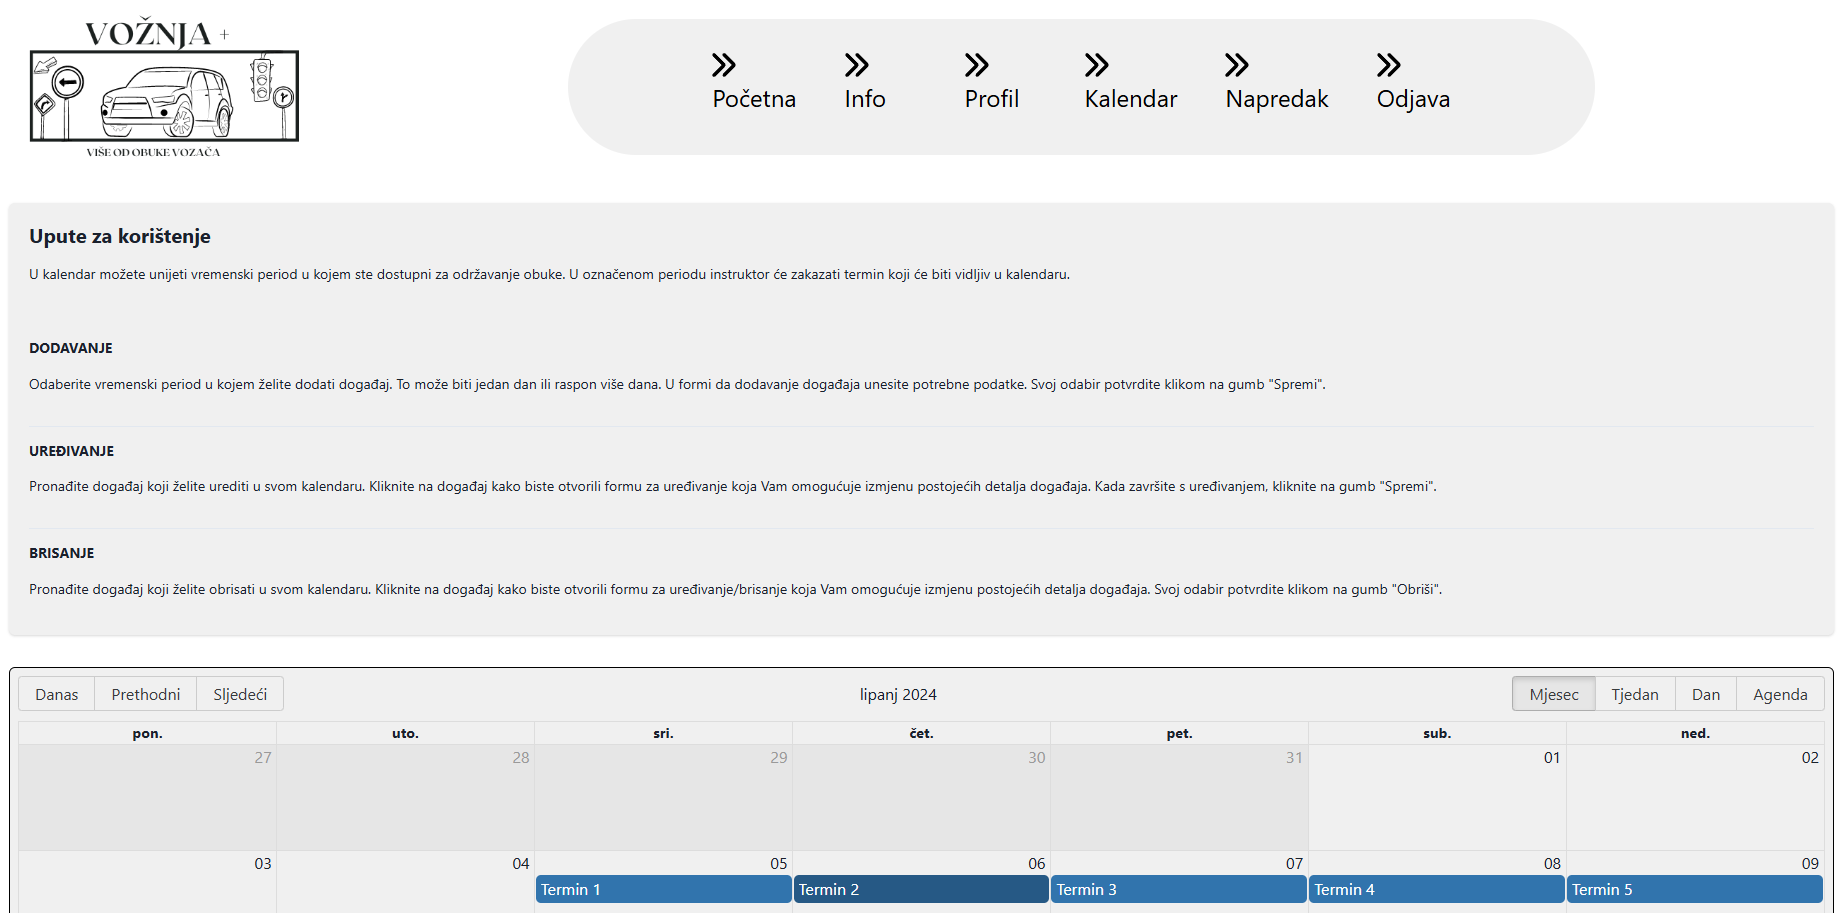
\includegraphics[width=\textwidth]{slike/kandidat2.png} 
					\centering
					\caption{Stranica s kalendarom}
					\label{fig:promjene}
				\end{figure}

    \begin{figure}[H]
					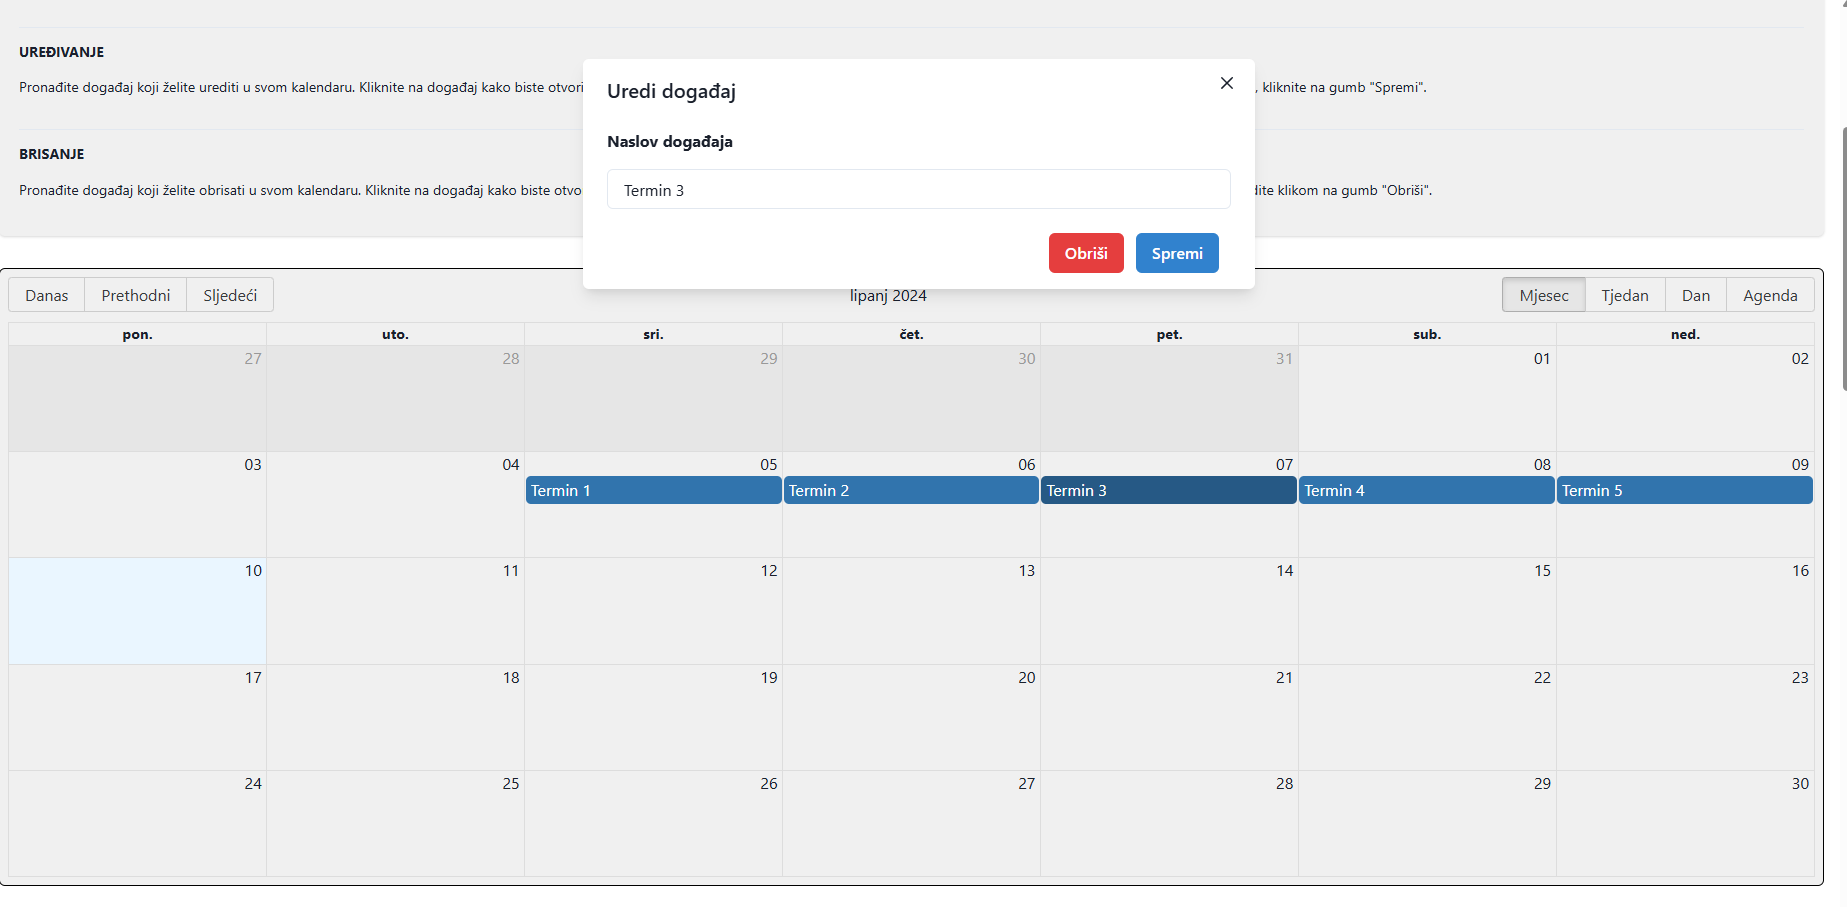
\includegraphics[width=\textwidth]{slike/kandidat3.png} 
					\centering
					\caption{Uređivanje događaja u kalendaru}
					\label{fig:promjene}
				\end{figure}

\noindent Za prikaz stranice napredak na slici 4.9. korisnik odabire opciju "Napredak" u navigacijskoj traci. Svaki predviđeni sat vožnje ima pripadajuću bilješku koja se može vidjeti na slici 4.10.

\begin{figure}[H]
					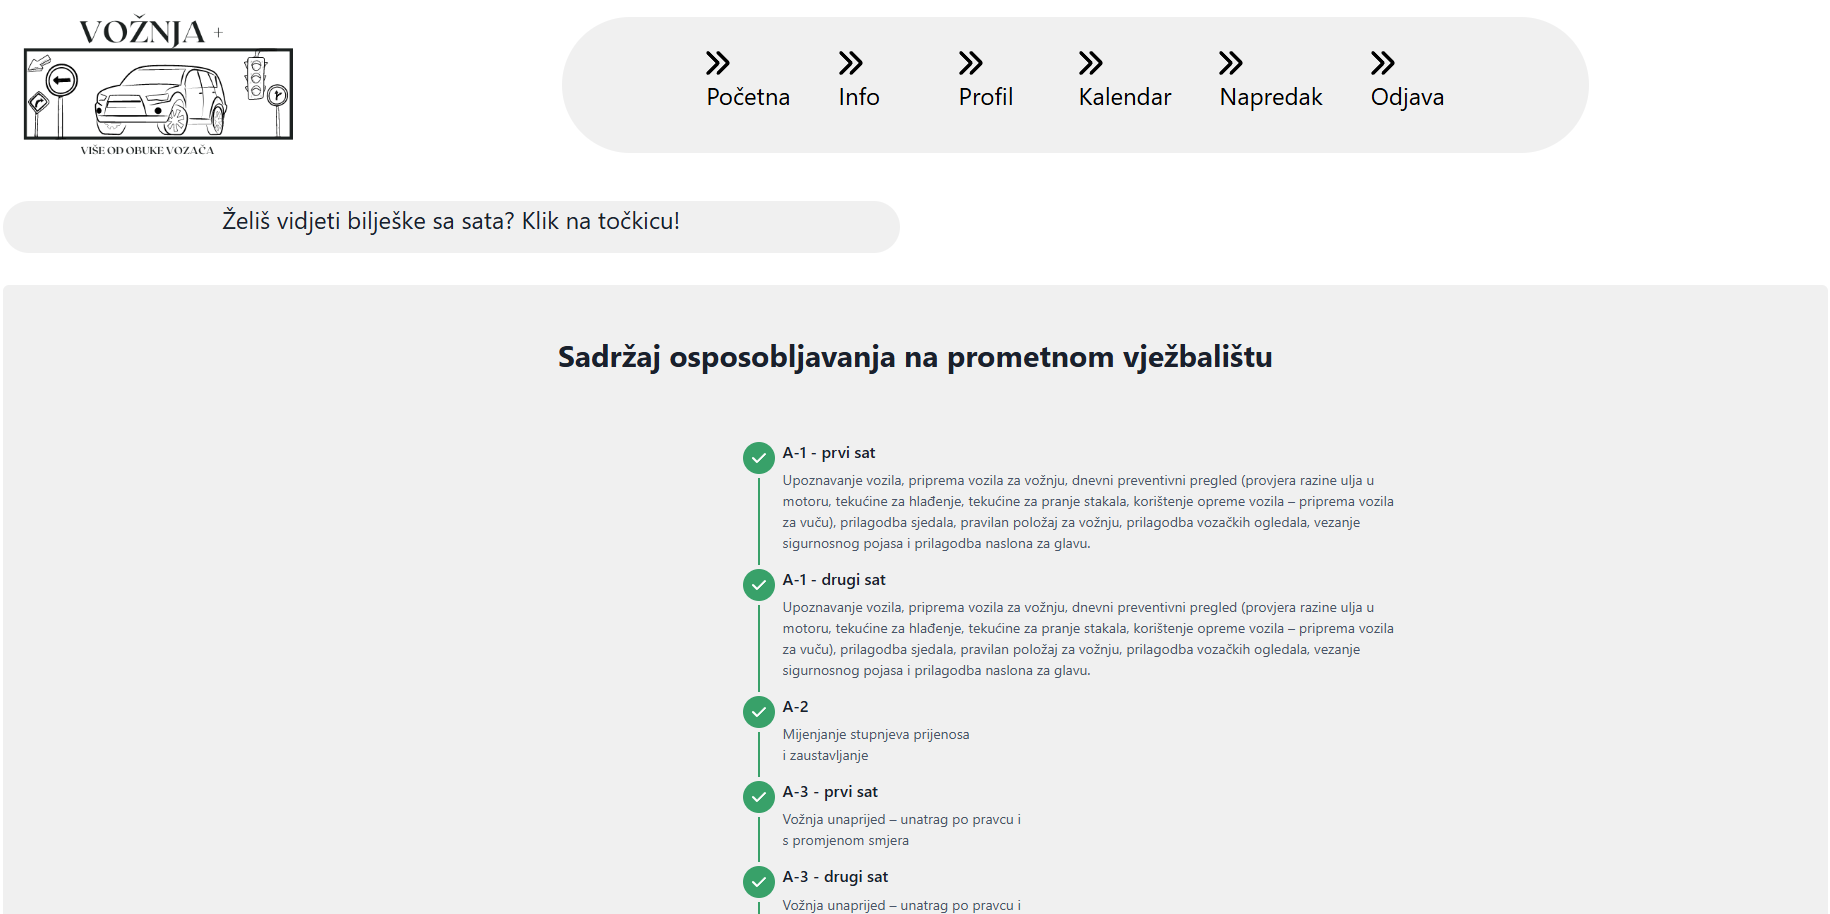
\includegraphics[width=\textwidth]{slike/kandidat4.png} 
					\centering
					\caption{Napredak stranica}
					\label{fig:promjene}
				\end{figure}

    \begin{figure}[H]
					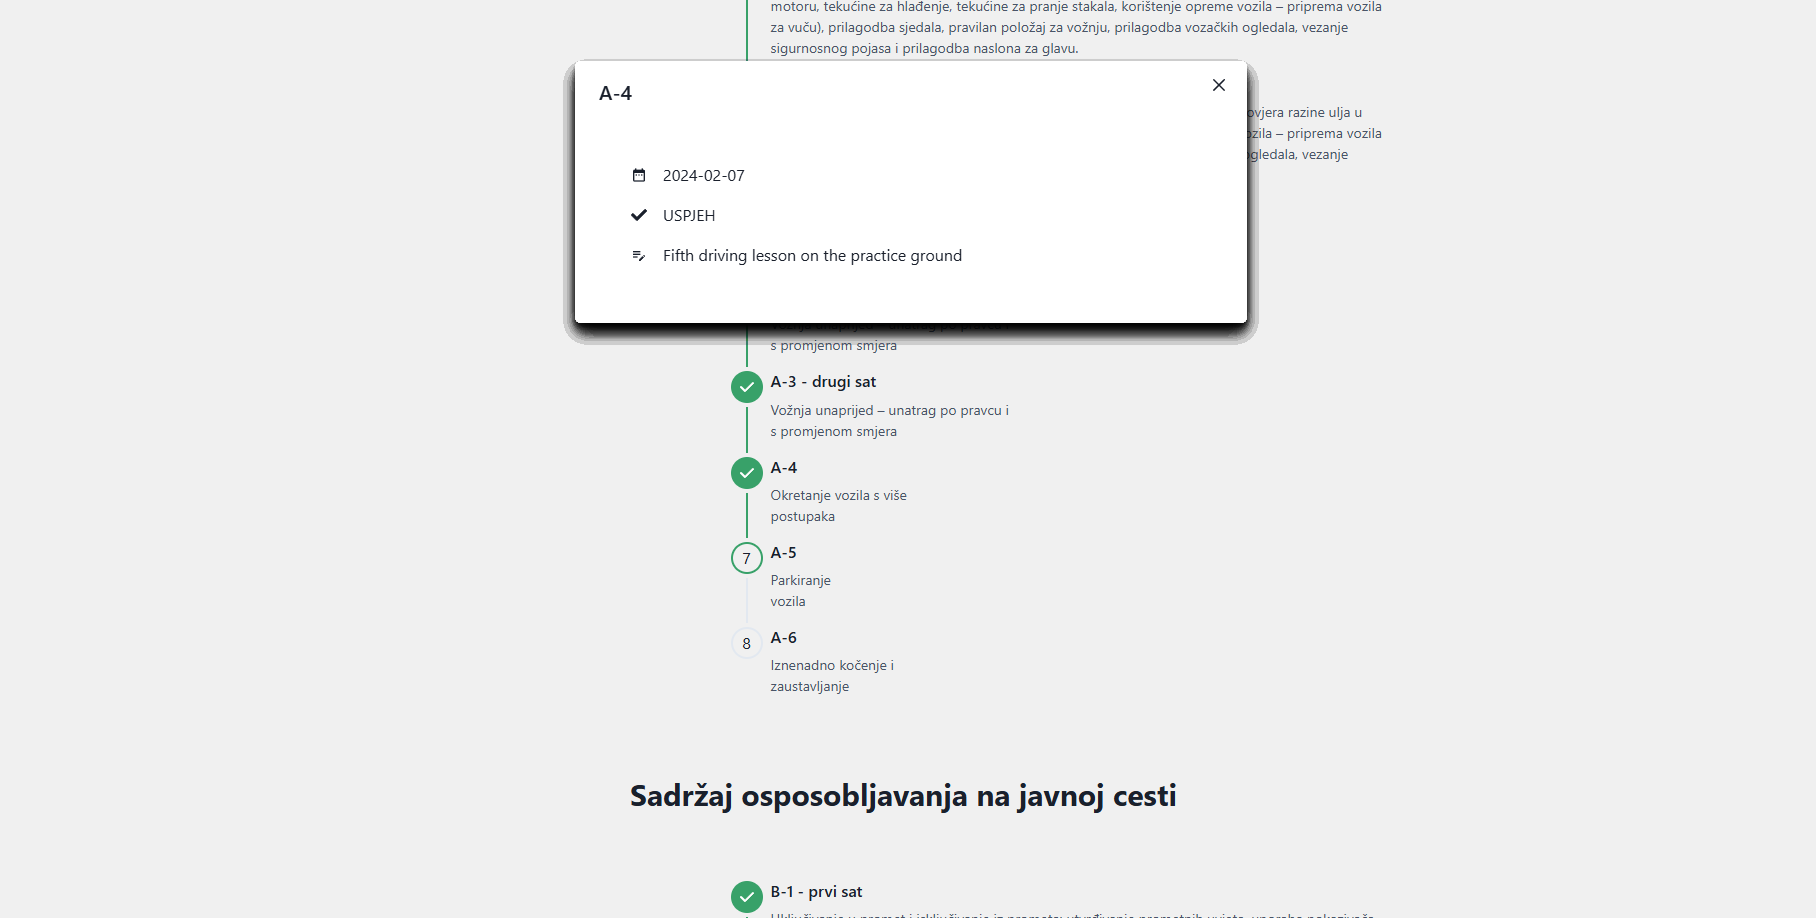
\includegraphics[width=\textwidth]{slike/kandidat5.png} 
					\centering
					\caption{Bilješka za sat}
					\label{fig:promjene}
				\end{figure}

\noindent \textbf{Sučelja instruktora autoškole }\\

\noindent Nakon što se instruktor prijavi u aplikaciju, pored osnovnih, omogućen mu je pristup dodatnim web stranicama. Na slici 4.11. možemo vidjeti kako izgleda stranica sa svim kandidatima kojoj mogu pristupiti instruktori i administratori.

\begin{figure}[H]
					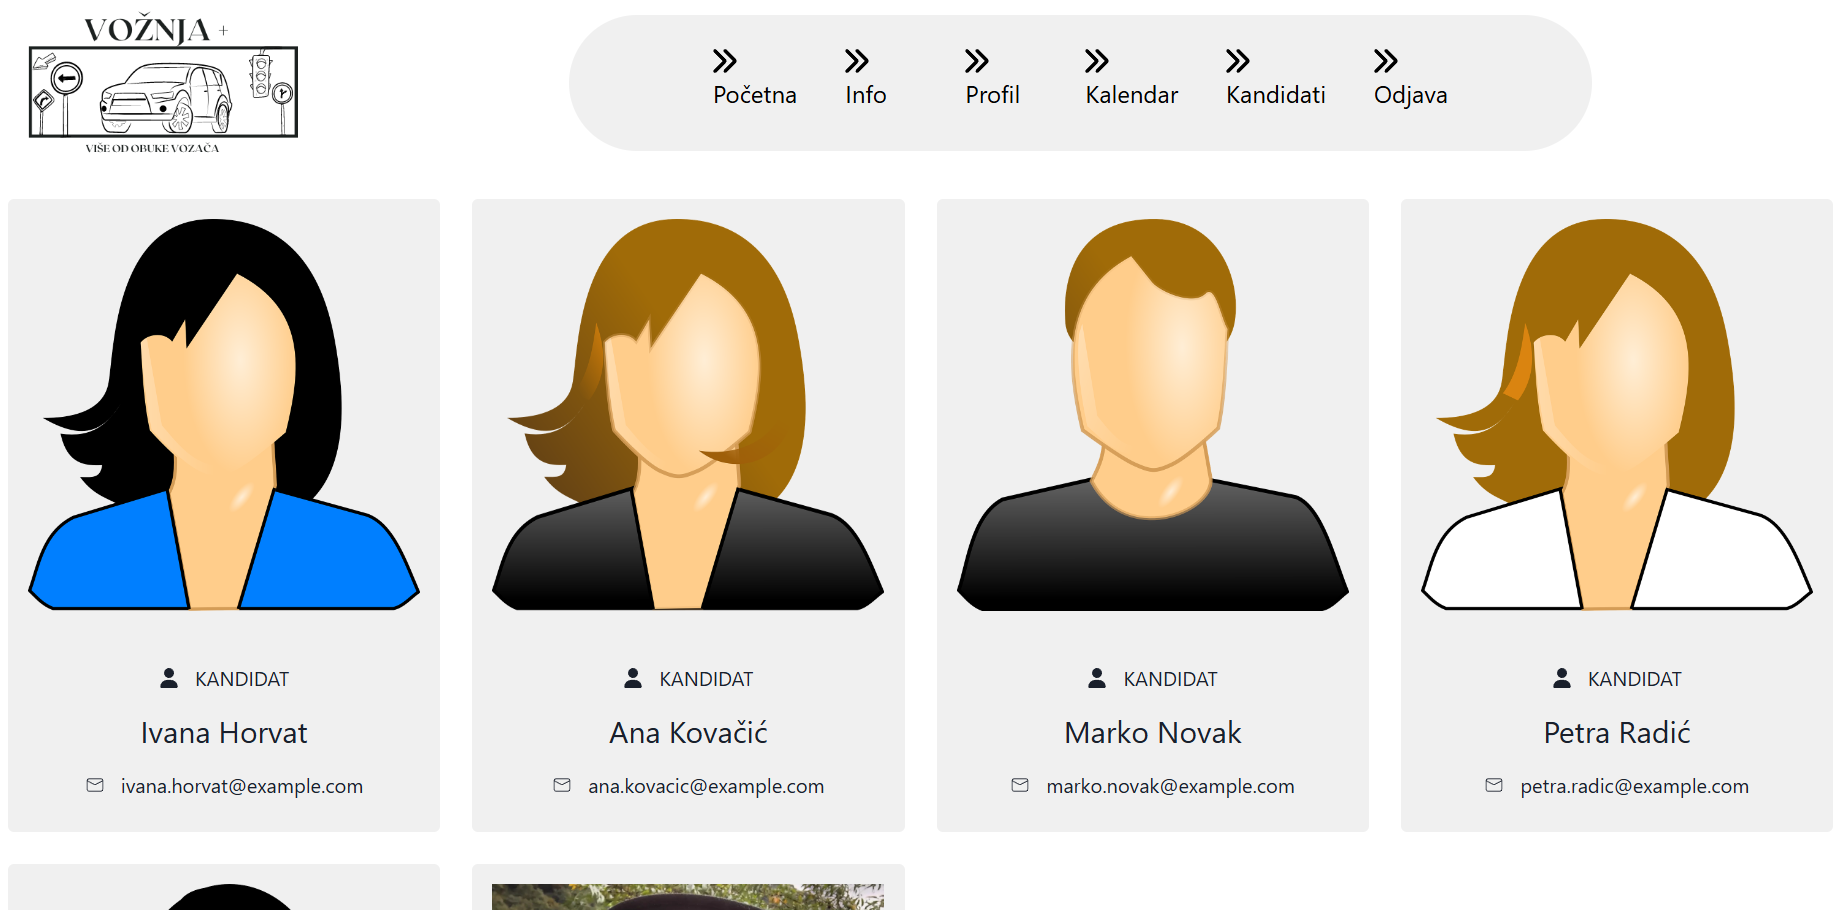
\includegraphics[width=\textwidth]{slike/instruktor1.png} 
					\centering
					\caption{Prikaz svih kandidata}
					\label{fig:promjene}
				\end{figure}

\noindent Nakon odabira na određenog kandidata iz prikaza prikazuje se stranica na slici 4.12. Putem prikazanog sučelja instruktor može pregledati kandidatov kalendar te u njega upisati, urediti ili obrisati termin. Osim toga, instruktor unosi bilješke za održani sat putem sučelja prikazanog na slici 4.13.

\begin{figure}[H]
					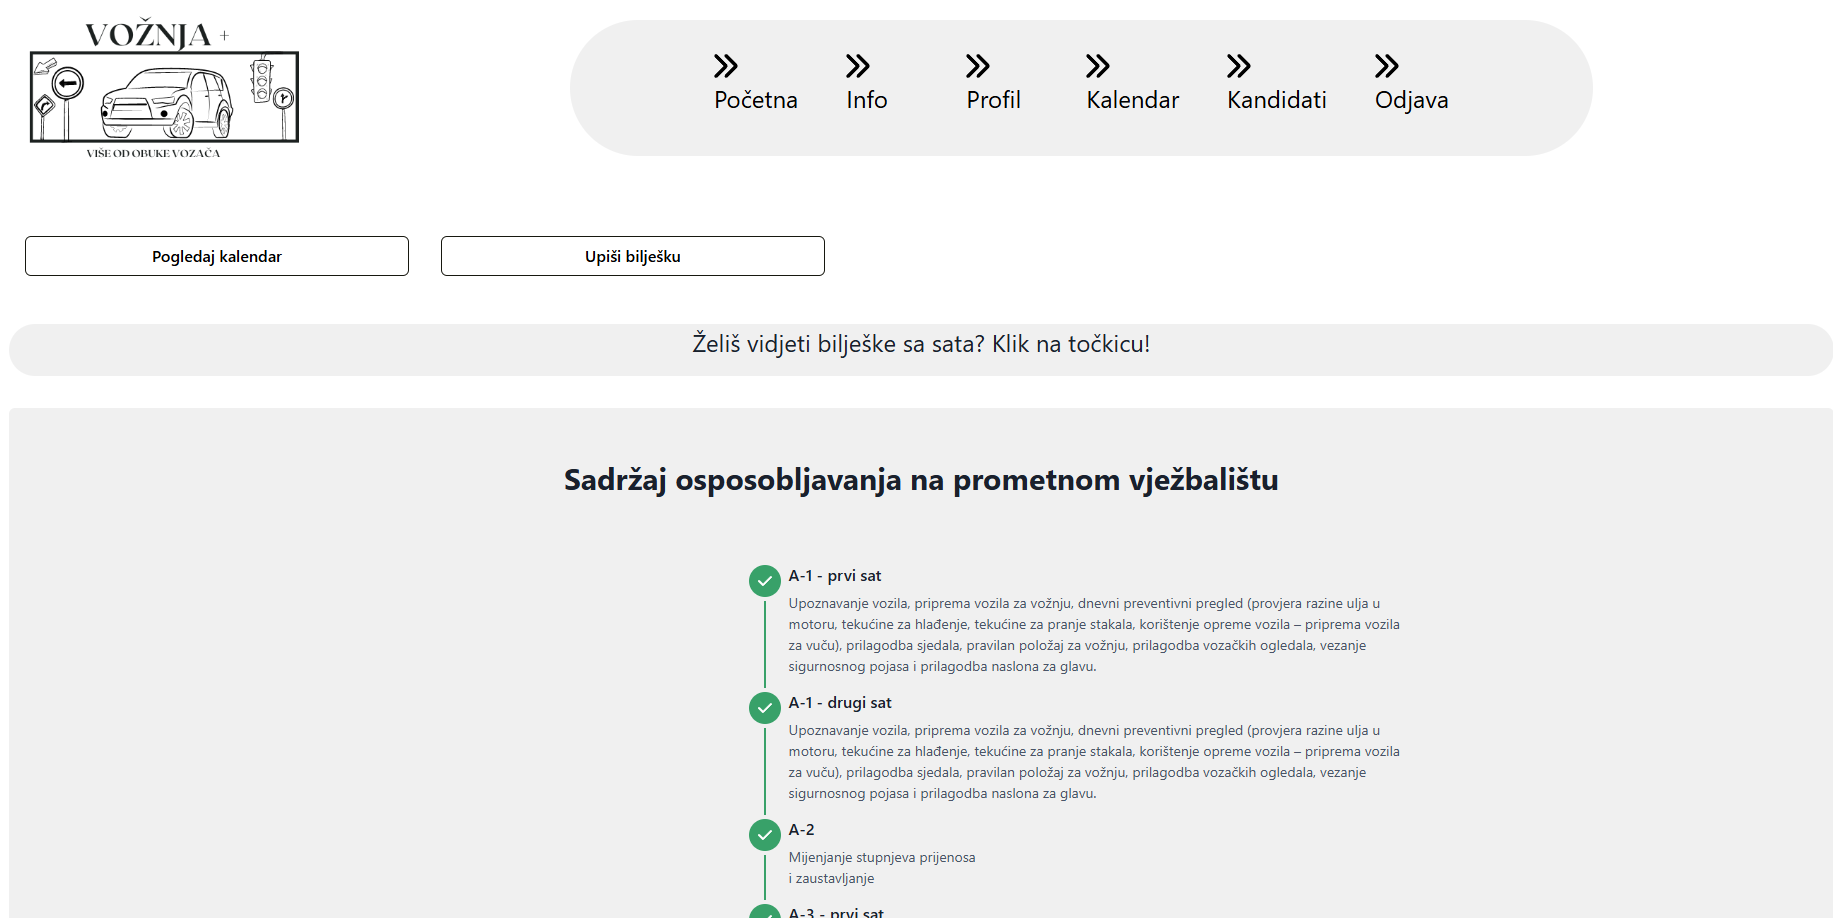
\includegraphics[width=\textwidth]{slike/instruktor2.png} 
					\centering
					\caption{Prikaz stranice za napredak}
					\label{fig:promjene}
				\end{figure}
\begin{figure}[H]
					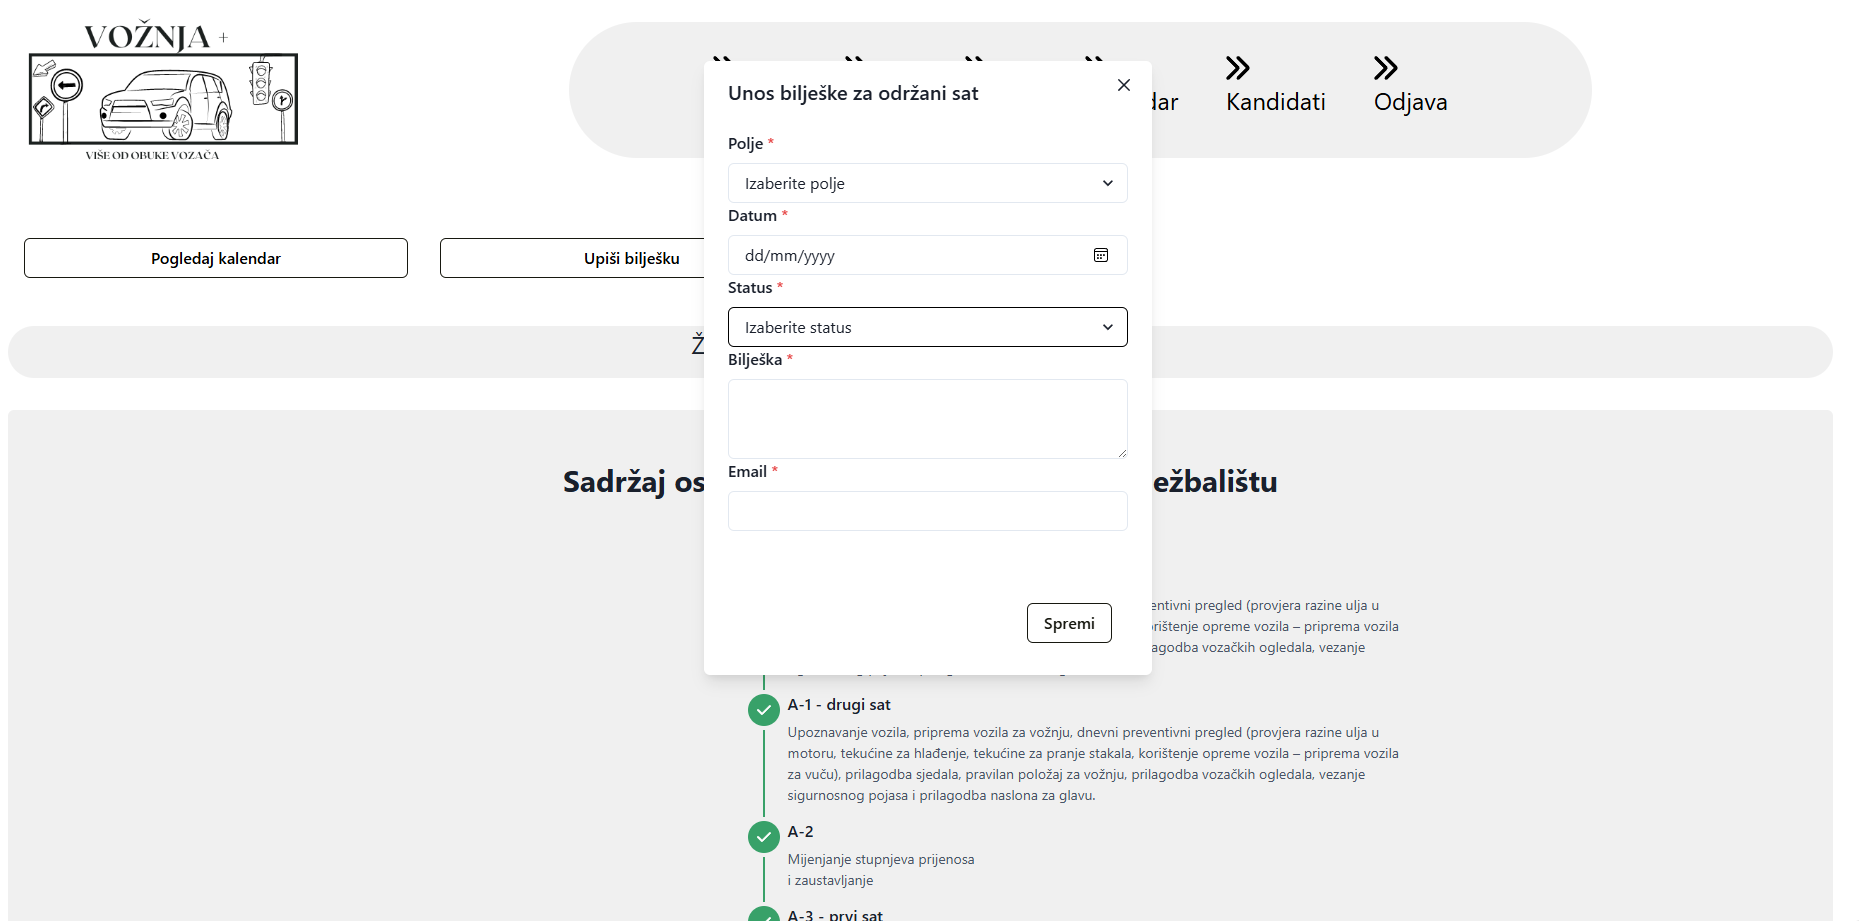
\includegraphics[width=\textwidth]{slike/instruktor3.png} 
					\centering
					\caption{Unos bilješke sa sata}
					\label{fig:promjene}
				\end{figure}

\noindent \textbf{Sučelja administratora autoškole }\\

\noindent Nakon što se administrator prijavi u aplikaciju, pored osnovnih, omogućen mu je pristup dodatnim web stranicama. Na slici 4.14. možemo vidjeti kako izgleda stranica koja prikazuje sve instruktore. Spomenutoj stranici može pristupiti samo administrator. Klikom na određenog instruktora prikazuje se stranica s kalendarom odabranog korisnika.

\begin{figure}[H]
					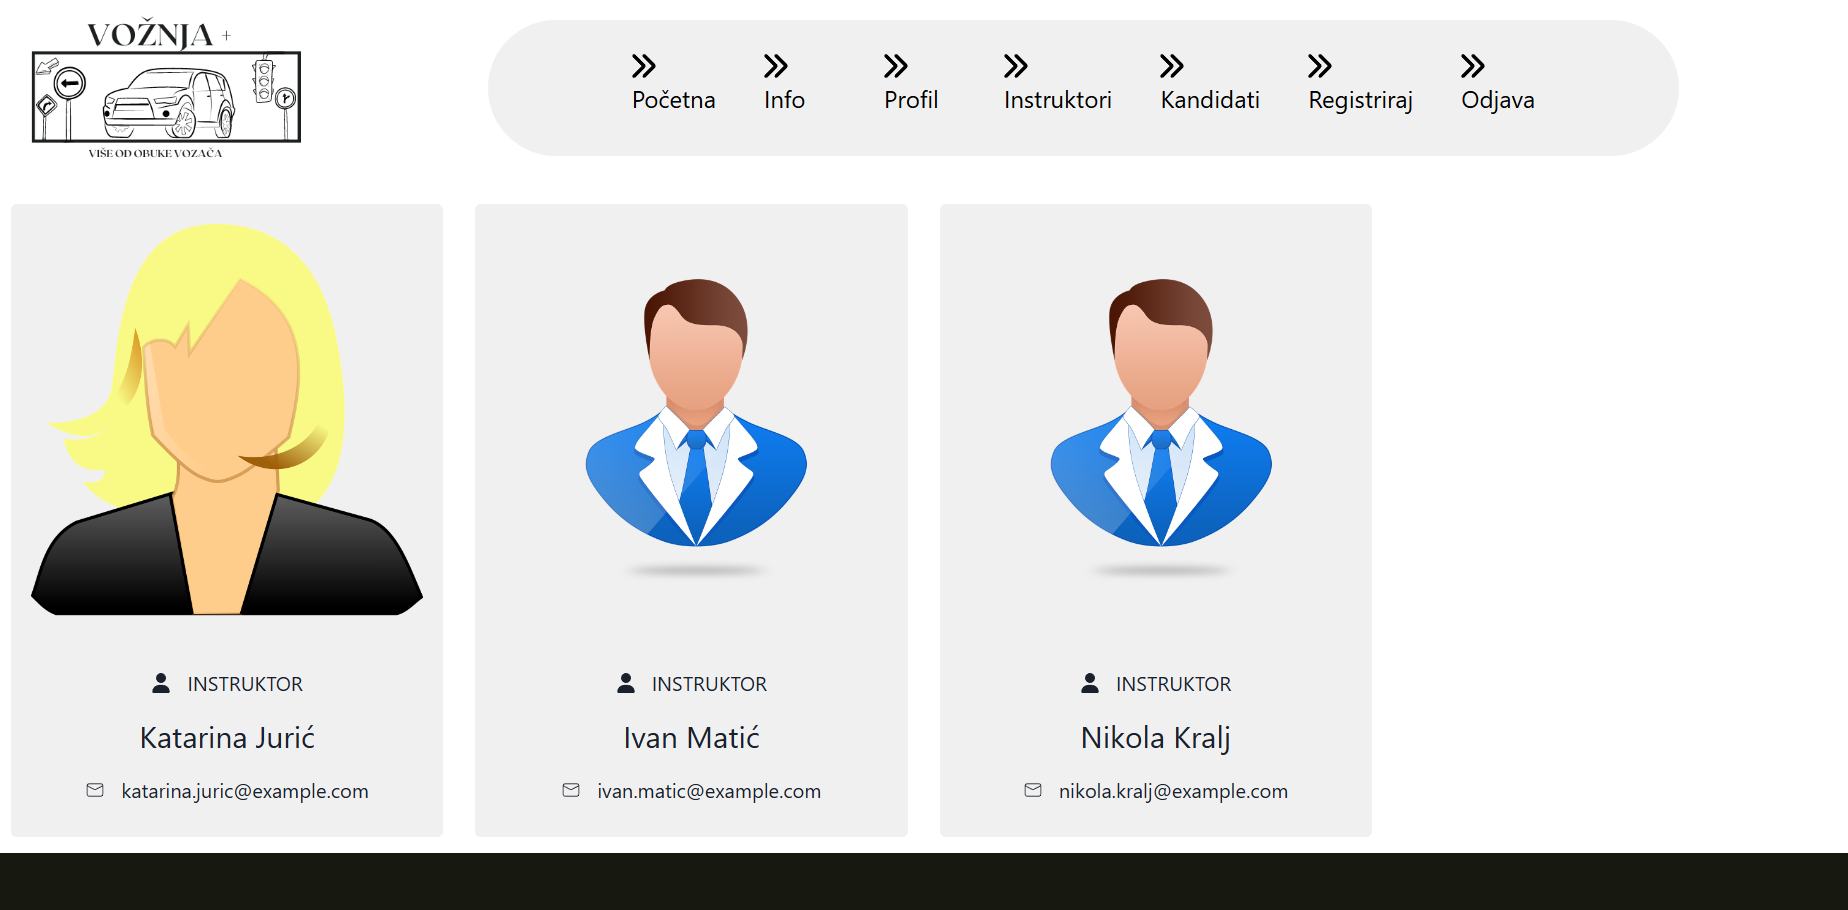
\includegraphics[width=\textwidth]{slike/admin1.png} 
					\centering
					\caption{Prikaz instruktora}
					\label{fig:promjene}
				\end{figure}

\noindent Na kraju, na slikama 4.15 i 4.16. možemo vidjeti prikaz forme za registraciju novih korisnika kojoj također može pristupiti isključivo korisnik s ulogom administratora. Na slici 4.16 vidi se i univerzalno podnožje svake stranice na kojem se mogu naći kontakt podaci.

\begin{figure}[H]
					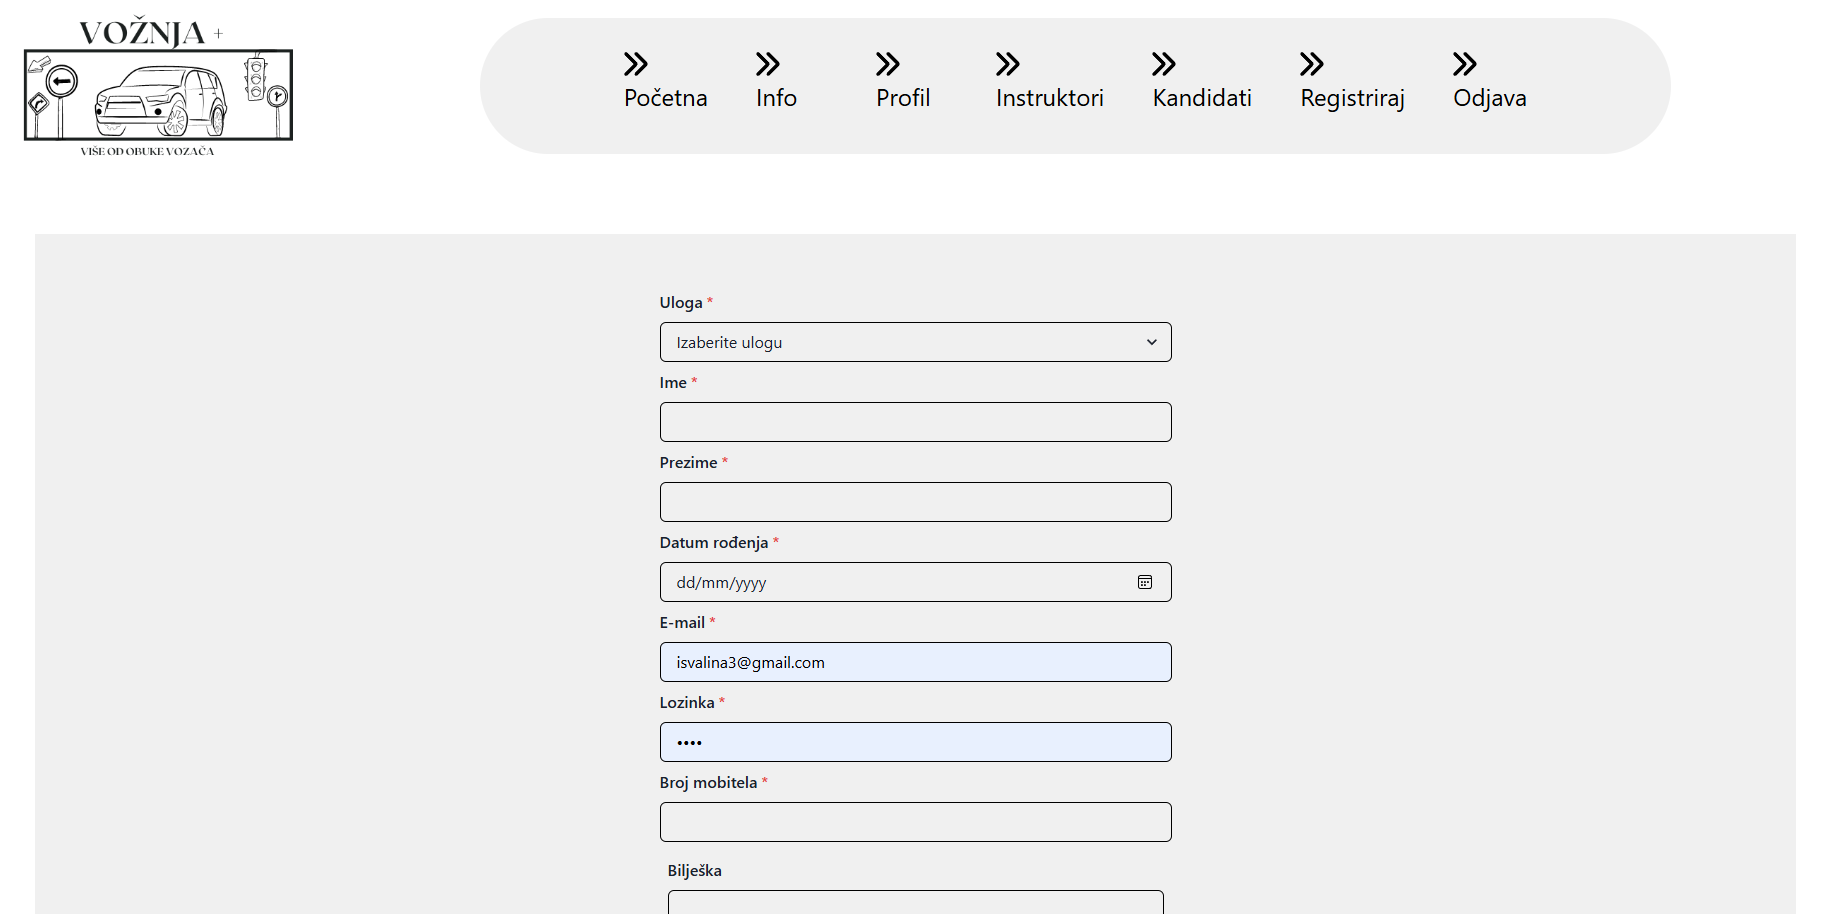
\includegraphics[width=\textwidth]{slike/admin2.png} 
					\centering
					\caption{Registracija novog korisnika}
					\label{fig:promjene}
				\end{figure}

    
\begin{figure}[H]
					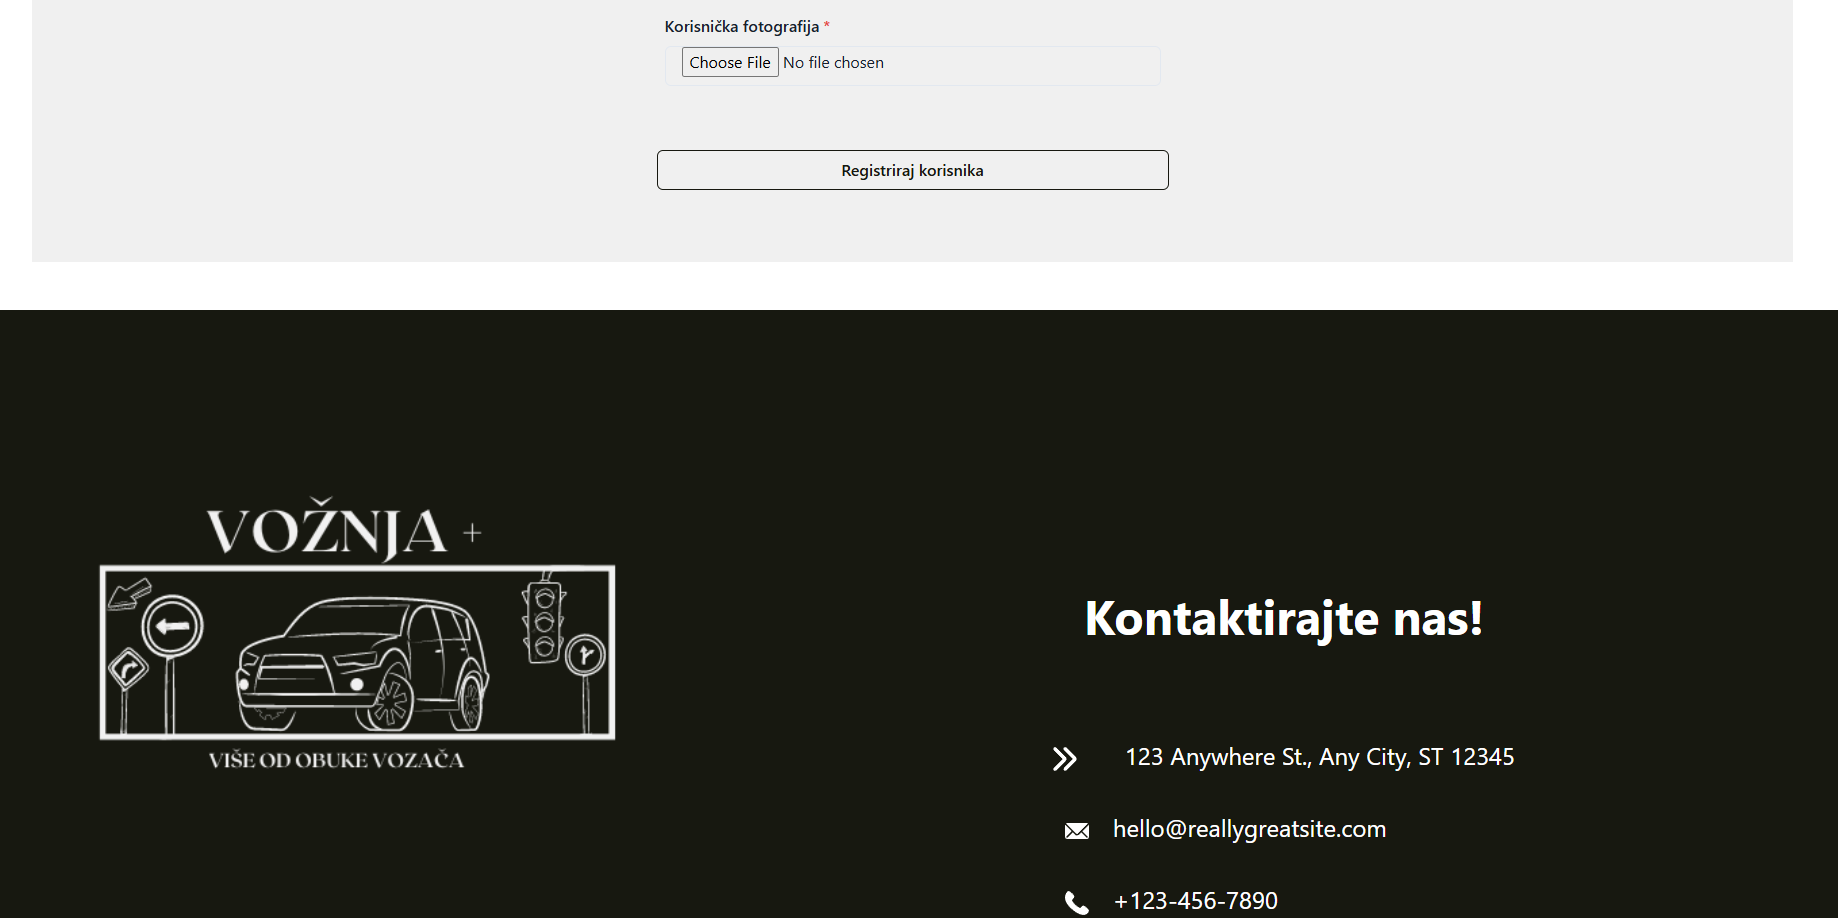
\includegraphics[width=\textwidth]{slike/admin3.png} 
					\centering
					\caption{Registracija novog korisnika i kontakt podaci}
					\label{fig:promjene}
				\end{figure}
    \chapter*{Zaključak}
\addcontentsline{toc}{chapter}{Zaključak}
\noindent U završnom radu izrađena je web aplikacija "Vožnja +" koja služi  za organizaciju i kontinuirano praćenje obuke za vozača B kategorije. Glavni cilj rada bio je cjeloviti razvoj  aplikacije koji se može podijeliti na tri glavna dijela: početak u kojem je dominantno bilo upoznavanje s novim tehnologijama s naglaskom na React, sredina u kojoj se primarno radilo na dizajnu sustava i odabirom arhitekture te implementacijski dio koji predstavlja najizazovniji dio cijelog projekta.

\noindent Uspješnoj realizaciji implementacijskog dijela znatno su doprinijeli kolegiji "Baze podataka", "Objektno orijentirano programiranje", "Razvoj programske potpore za web", ali i široka programerska zajednica koja je ključna za dijeljenje znanja i resursa, ali motivacije i podrške. Najvažnije funkcionalnosti aplikacije su praćenje obuke kandidata bilježenjem svakog održanog sata, ali i kalendar koji ima mogućnost sinkronizacije između instruktora i kandidata što doprinosi boljoj organizaciji obuke, ali i praćenju radnog opterećenja instruktora. Osnovne funkcionalnosti aplikacije obogaćene su integracijom servisa Cloudinary i EmailJS koje omogućuju rad s multimedijskim sadržajem i komunikaciju elektroničkom poštom. 

\noindent Aplikacija ima potencijal za brojna unapređenja od kojih se posebno izdvaja integracija s postojećom aplikacijom za savladavanje teorijskog dijela obuke. Riječ je o aplikaciji "Autoškola" koja služi  za treniranje kandidata za polaganje ispita iz prometnih propisa. Slanje automatskih podsjetnika za termine u kalendaru putem elektroničke pošte također bi bilo značajno poboljšanje. Ako bi se sustav koristio u praksi, aplikacija ima mogućnost unapređenja sigurnosti sustava. Osim toga, postoji i mjesto za napredak u izgledu aplikacije i poboljšanju arhitekture cjelokupne aplikacije.
    \chapter*{Literatura}
\addcontentsline{toc}{chapter}{Literatura}

\begin{enumerate}

    \item Astah Community, \emph{Astah Community}, (n.d.). Poveznica: \url{http://astah.net/editions/uml-new}; pristupljeno u lipnju 2024.

    \item Chakra UI, \emph{Getting Started with Chakra UI}, (n.d.). Poveznica: \url{https://v2.chakra-ui.com/getting-started}; pristupljeno u svibnju 2024.

    \item EmailJS, \emph{EmailJS ReactJS}, (n.d.). Poveznica: \url{https://www.emailjs.com/docs/examples/reactjs/}; pristupljeno u svibnju 2024.

    \item JSON Web Tokens (JWT), \emph{Introduction to JSON Web Tokens}, (n.d.). Poveznica: \url{https://jwt.io/}; pristupljeno u svibnju 2024.

    \item Nastava iz predmeta Upravljanje vozilom, \emph{Instruktor vožnje}, (n.d.). Poveznica: \url{https://www.instruktor-voznje.com.hr/nastava_iz_predmeta_upravljanje_vozilom/}; pristupljeno u travnju 2024.

    \item Spring Boot Project, \emph{Spring Boot Project}, (n.d.). Poveznica: \url{https://spring.io/projects/spring-boot}; pristupljeno u svibnju 2024.

    \item Spring Boot H2 Database, \emph{Spring Boot H2 Database}, (n.d.). Poveznica: \url{https://www.baeldung.com/spring-boot-h2-database}; pristupljeno u svibnju 2024.

    \item Programsko inženjerstvo, \emph{FER ZEMRIS}, (n.d.). Poveznica: \url{https://www.fer.unizg.hr/predmet/proinz}; pristupljeno u svibnju 2024..

    \item React Big Calendar, \emph{React Big Calendar}, (n.d.). Poveznica: \url{https://github.com/jquense/react-big-calendar}; pristupljeno u lipnju 2024..

    \item React Documentation (Legacy), \emph{React Documentation (Legacy)}, (n.d.). Poveznica: \url{https://legacy.reactjs.org/}; pristupljeno u lipnju 2024.

\end{enumerate}

    \include{Sažetak}
    \chapter*{Summary}
\addcontentsline{toc}{chapter}{Summary}
\noindent This thesis consists of the "Vožnja +" web application and the accompanying documentation.\

\noindent The development of the web application for driving schools was realized through three phases: defining user requirements and acquiring competencies, designing the system and selecting the application architecture, and implementation within the Spring Boot and React frameworks. The main functionalities of the application are organizing training sessions using a calendar and tracking progress through a predefined training structure and notes entered for each session. The Cloudinary service for media content manipulation is integrated into the backend part of the application, while sending emails is enabled through the EmailJS service in the frontend part of the application. The database layer is implemented using the H2 relational database. Each step is thoroughly documented, and the final appearance of the application is presented.\

\noindent The result of the work is an efficient organizational system that facilitates instructors and driving school students in organizing and tracking the progress of driver training for category B. The application has the potential for numerous enhancements, particularly the integration of various educational content for self-learning, similar to the existing "Autoškola" application used for mastering the theoretical part of the training. Additionally, it is possible to expand its functionalities by including training for other vehicle categories. Although the application is specifically tailored for driving schools, it can be developed into a general system for organizing and tracking progress during learning.

\vspace{1cm}
\noindent Keywords: driving school, Spring Boot, React, H2, Cloudinary, EmailJS

\end{document}
